% ===========================================================================
% v2 REWRITE (2026-08-10, Vikas-approved outline: REWRITE_OUTLINE_v2.md).
% v1 (agentic_grb.tex) PRESERVED untouched until the swap is approved.
% Spine = docs/agentic_workflow_map.md (the collaborator page).
% Nomenclature policy: NO internal filenames; paper names per the outline table
%   (Skill Library, Campaign Protocol, Reconciliation Protocol, Lesson Test-Suite,
%    Burst Records, Campaign Ledger, validity gates, ...).
% Numbers policy: real walkthrough-era values ONLY, each \prov-flagged; refreshed
%   mechanically at the frozen production sweep. No invented numbers, ever.
% ===========================================================================
\documentclass[twocolumn]{aastex631}
\usepackage{tikz}
\usetikzlibrary{positioning,arrows.meta,shapes.geometric}
\tikzset{
  box/.style={draw, rounded corners=2pt, align=center, font=\scriptsize, inner sep=3pt, minimum height=14pt},
  gate/.style={box, fill=black!8, thick},
  hum/.style={box, fill=black!15},
  dec/.style={diamond, aspect=2.4, draw, align=center, font=\scriptsize, inner sep=1pt},
  arr/.style={-{Stealth[length=5pt]}, semithick},
  lab/.style={font=\tiny, midway}
}

\newcommand{\PENDING}[1]{\textbf{\textcolor{red}{[PENDING run: #1]}}}
\newcommand{\TODOcite}[1]{\textbf{\textcolor{blue}{[cite: #1]}}}
\newcommand{\prov}{\textsuperscript{(p)}}
\newcommand{\ac}[1]{\parbox[t]{5.3cm}{\raggedright #1}}   % authority-table cell (v3 §3)
\newcommand{\rc}[1]{\parbox[t]{10.2cm}{\raggedright #1}}  % register-table cell (v3 §5)
\newcommand{\nc}[2]{\parbox[t]{#1}{\raggedright #2}}       % needs-table cell (v3 §10)   % provisional walkthrough-era number
\newcommand{\Ep}{E_{\rm p}}
\newcommand{\kT}{kT}

\shorttitle{Can AI Agents Analyze GRBs?}
\shortauthors{Chand et al.}

\begin{document}

% --- TITLE: Vikas to pick; option B (v1) kept below ------------------------
\title{Can AI Agents Analyze Gamma-Ray Bursts?}
% \title{Can Agentic AI Do Gamma-Ray Burst (GRB) Analysis?
% A Human-versus-Agent Benchmark on Time-Resolved \textit{Fermi}/GBM Spectroscopy}

\author{Vikas Chand}
\affiliation{Louisiana State University, Baton Rouge, LA, USA}
\email{vikas.chand.physics@gmail.com}

\author{Khushboo Sharma}
\affiliation{Aryabhatta Research Institute of Observational Sciences (ARIES), Nainital, India}

\author{Jagdish C. Joshi}
\affiliation{Aryabhatta Research Institute of Observational Sciences (ARIES), Nainital, India}

% PROVISIONAL abstract (r5, 2026-09-03; PI: "just write something, and abstract can anyway be written at the end when paper is done")
\begin{abstract}
Time-resolved spectroscopy of gamma-ray bursts (GRBs) rests on judgement
calls: which detectors to trust, where the background lies, where the
burst begins and ends, how finely to bin it, and which of two dozen
spectral models to adopt. We describe the design of an agent that makes
those calls under human approval, and what it caught on its first burst.
A language model runs inside a harness of deterministic tools,
plain-language skill documents, state derived from disk, and enforced
boundaries; a producer never verifies its own work. The agent analyses
each burst blind, freezes its numbers before it reads the published
literature, and turns every mismatch into a numbered lesson with an
executable test. Applied to a campaign of 106 single-pulse
\textit{Fermi}/GBM bursts, the design fits a 24-model menu to every time
bin and assembles reports whose numbers recompute from the products on
disk; on the first burst walked end to end it caught engine defects, now
fixed and tested, and confirmed blind predictions while refuting one.
The trained artifact is the skill library, readable by a student or by
another AI system, which we release with the engine, the tests, and the
per-burst records.
\end{abstract}

\keywords{Gamma-ray bursts (629) --- Astronomy data analysis (1858) ---
Astronomy software (1855) --- Astrostatistics (1882)}

% ===========================================================================
\section{Introduction} \label{sec:intro}
% ===========================================================================

The question in our title is usually asked as if it had a yes-or-no answer.
It does not, because ``AI doing analysis'' names at least two different
architectures, and the difference between them decides what the answer can
mean. In the first architecture, a \emph{workflow}, the analysis follows
predefined paths---the same stages, in the same order, for every burst---and
software executes them. In the second, an \emph{agent}, a model directs its
own process: it decides what to do next, which tools to call, and when it is
finished \citep{anthropic2024agents}. Workflows are auditable and dull; agents are
flexible and hard to trust. Most claims that ``AI analyzed the data'' blur
the two.

This paper builds and tests a deliberate hybrid, and names it honestly: a
\emph{gated workflow with bounded agency}. The analysis pipeline---data
acquisition, detector and background selection, adaptive binning, spectral
fitting, temporal analysis, quality control---is a workflow: its stages are
fixed, its statistics are chosen in advance, and its outputs are stamped
with provenance. Inside that workflow, an AI exercises agency at exactly the
points where judgement is required and we can afford to audit it: which of
twenty-four spectral models wins a gated comparison, whether a fit is valid
or sits on a parameter rail, whether a published value has been verified at
its source, and---when our numbers disagree with the literature---whether the
fault is ours, theirs, or a difference of analysis frames. A human approves
every step before the next one runs. Nothing advances on silence, and no
approval is ever fabricated: every decision carries a stamp naming who, or
what, made it.

Why is time-resolved GRB spectroscopy the right testbed rather than a
convenient one? Because it concentrates, in one measurement problem, the
three features that make scientific AI hard to evaluate. First, the
decisions have no answer key. Two careful published analyses of the same
burst, using overlapping data and defensible methods, can disagree about
whether a thermal component exists at all; the literature is a
\emph{distribution} over defensible choices, not a ground truth
\citep{2022ApJ...938..159S,2019ApJ...887...13F}. Second, the instrument
matters: responses age, detectors are occulted, backgrounds are fit, and a
systematic that is invisible in one regime of burst brightness or hardness
appears only when the sample happens to present the other. Third, the
stakes are population-level: our science application is a census of
spectral shapes across 106 single-pulse bursts selected morphologically
\citep{2024ApJ...972...83B}, and a small per-burst bias becomes a
population-level artifact. A system that merely \emph{runs} on such data is
easy; a system whose outputs deserve trust must show its work at every one
of these pressure points.

Our design answer, developed in \S\ref{sec:workflow}, has one unusual
component that we believe is the paper's main methodological contribution.
The system's procedural knowledge lives in a \emph{Skill Library}: versioned,
plain-language documents---one per pipeline stage---that state how the stage
is run, what its known failure modes are, and what was learned from every
burst that ever taught it something. The Library is executable culture: an
AI agent reads the same document a new student would, and both are bound by
the same rules. Around the Library sits the second component: a roster of
single-purpose specialist agents---each defined by its role, the skills it
reads, and the domain tools it commands (\S\ref{sec:roster})---and an
operating skeleton of typed states, typed failures, and mechanical gates
that makes their fan-out and reassembly auditable (\S\ref{sec:skeleton}).
Crucially, the Library \emph{learns} under a discipline we
call lessons-as-tests: a lesson enters the Library only as a claim with
provenance (which burst, which date, which evidence) \emph{and} an
executable test that fails if the lesson is ever violated again. Weights
are never updated; the harness is. \S\ref{sec:learning} shows what this
training regime produced over the first ten bursts of the campaign,
including its learning curve, and \S\ref{sec:verify} develops the
verification doctrine---blind-first analysis, frozen predictions, and an
independence requirement we state as: agreement between two analyses is
evidence only in proportion to how deep their shared primitives go.

We are not the first to ask whether AI can do science end-to-end.
Multi-agent systems now generate ideas, run analyses, and draft papers
across disciplines \citep{2025arXiv251026887V,2025arXiv250408066Y}. Our design differs in direction: where those
systems are breadth-first---an agent writes fresh analysis code for each
project---ours is depth-first: the agents operate a single, tested,
domain-specific engine, and the system's growth is the accumulation of
verified domain lessons rather than of generated artifacts. The comparison
is instructive in both directions, and we return to it in
\S\ref{sec:discussion}: the breadth-first systems demonstrate, at scale,
exactly the evaluation gap---qualitative review standing in for ground
truth---that our gated, decision-level scoring is designed to close.

The paper is organized as follows. \S\ref{sec:sample} describes the sample
and data. \S\ref{sec:workflow} presents the architecture: the Campaign
Protocol, the Skill Library, the specialist roster and its domain tools,
the authority split between workflow, agent, and human, the doctrine
distilled from its failures, and the operating skeleton that enforces it.
\S\ref{sec:learning} presents harness learning and the campaign learning
curve. \S\ref{sec:verify} presents the verification doctrine and the
adversarial experiments. \S\ref{sec:design} describes the human-versus-agent
benchmark design. \S\ref{sec:results} reports walkthrough-era results, all
provisional\prov{} until a frozen production sweep. \S\ref{sec:discussion}
discusses limits, and \S\ref{sec:conclusions} concludes. Throughout,
walkthrough-era numbers carry the flag\prov{}; they will be regenerated
mechanically when the converged pipeline is frozen and run once over the
full sample.

% ===========================================================================
\section{Sample and Data} \label{sec:sample}
% ===========================================================================
% [KEEP from v1 with light compression: 106 single-pulse GBM bursts,
%  morphological selection; TTE/CSPEC/RSP2/POSHIST + LLE/LAT where present;
%  data quality (never detection significance) as the inclusion gate.]
\PENDING{port v1 \S2 with the L17 inclusion-gate paragraph added}

% ===========================================================================
% ---- v3 architecture block (decision 20): §3 + §4 from fragments; v2 §3 (202-504) replaced; see
% ---- paper_agentic/v3/DECISION_SHEET_architecture_block.md §3 for where every v2 paragraph went.
% ===========================================================================
% v3 §3 — THE HARNESS, COMPONENT BY COMPONENT (replaces v2 §3 "The Agentic Workflow")
% Census commit for every count marked \prov: 4df6884 (roster T1, commit 427fdc5).
% Figure F1 = paper_agentic/figures/fig_F1_harness_anatomy (gated; sha d355cbec…).
% Table T1 = paper_agentic/v3/tab_T1_roster.tex (generated from the roster; appendix).
% v2 text that MOVES rather than dies: "Inside the fitting step" -> §4 (with F3);
% "Two planes" -> §6; "The doctrine" -> §5; the register + hierarchy paragraphs of
% "The operating skeleton" -> §5; the state/cascade paragraphs -> §3.4 below; the
% authority table -> §3.5 below. Nothing is cut without a later chng that shows where it went.
% ===========================================================================
\section{The Harness, Component by Component} \label{sec:harness}

We use one vocabulary throughout. The \emph{model} is the language model we
call; it reasons, and it has no memory between calls and no way to check
its own claims against the world. The \emph{harness} is everything around
that call that lets the system act and keeps it honest. Recent engineering
accounts of agent harnesses\footnote{Bowne-Anderson, ``How to build an
effective agent harness'' (2026); B\"ockeler, ``Harness engineering for
coding agent users'' (2026); the Palantir Ontology documentation; and two
vendor posts. URLs in the provenance manifest.} converge on five runtime
jobs: run the reasoning loop, execute tools, assemble and manage context,
persist state, and enforce boundaries. Figure~\ref{fig:anatomy} lays our
system out under those five jobs, drawing each component solid where it
exists on disk and dashed where it is only proposed. Table~\ref{tab:roster}
(Appendix~\ref{app:roster}) states the work of every component in one
sentence, with its origin quoted and dated. The counts in this section are
taken at one commit\prov{} and will move; the roster says which commit.

\begin{figure*}[t]
\centering
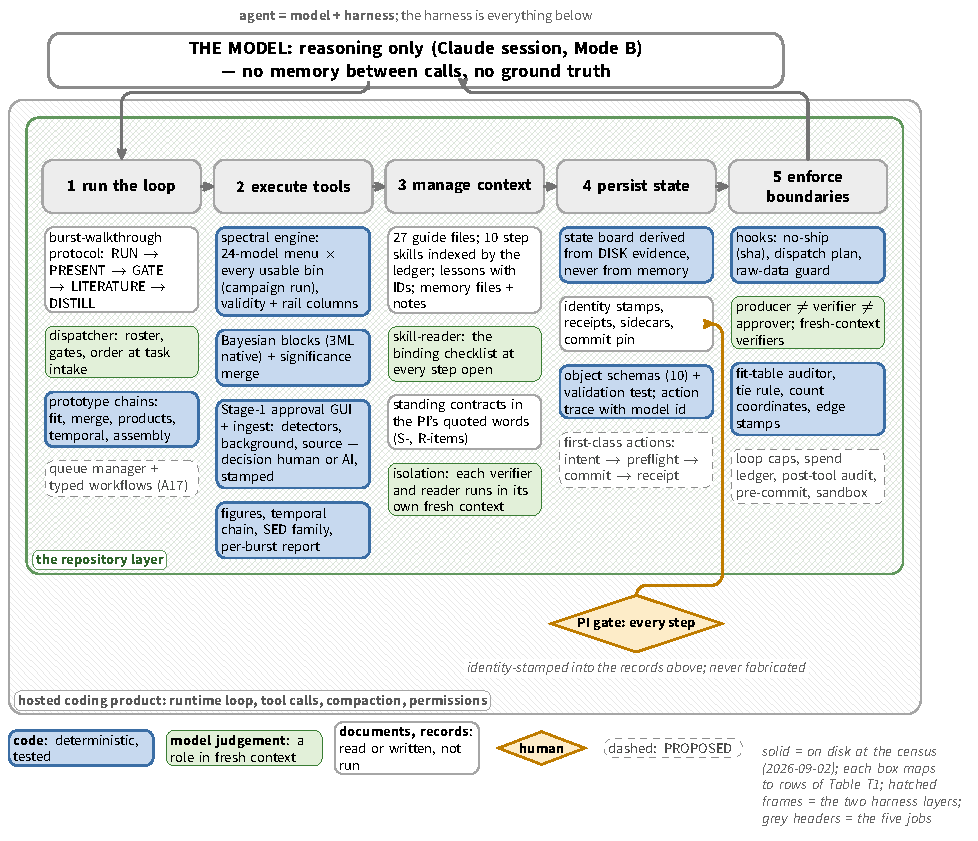
\includegraphics[width=\textwidth]{figures/fig_F1_harness_anatomy.pdf}
\caption{The harness anatomy. The five runtime jobs of an agent harness,
with the components this campaign has under each. Solid boxes exist on
disk at the census commit; dashed boxes are proposed in the requirements
register but not yet built. The human gate stamps every step with an
identity; approvals are never generated on the human's behalf. Each box
maps to rows of Table~\ref{tab:roster}.}
\label{fig:anatomy}
\end{figure*}

\subsection{The loop and the state machine} \label{sec:loop}

The reasoning loop today is the interactive session of a commercial coding
harness, which we call Mode~B: the harness supplies the loop, the tool
execution, the compaction of long context, and a permission layer, and our
repository supplies everything that makes the session a GRB analyst. The
per-burst protocol drives that loop: each of the eleven steps of the burst
ledger is run, presented to the human in a fixed four-sentence form, gated,
compared with the literature where the step calls for it, and distilled
before the next step starts. A \emph{dispatcher} reads each task and the
requirements register at intake and returns the agents, gates, and order the
task requires, naming every guard that does not yet exist. The loop is
stateful only through the disk: a burst occupies one of fourteen typed
states\prov{} (thirteen from ingested to closed, plus one terminal
exclusion), and the state is derived from the products on disk at read
time, never asserted by the session.

Two parts of the loop are declared debt. The queue manager that would own
campaign sequencing, hold the memory-budget claims, and resume after a
kill, and the eleven typed workflows\prov{} that would run each state
transition as a fixed sequence of reader, producers, verifiers, and stamps,
are specified in the skeleton document and not built; transitions run today
on prototype shell chains that invoke no agent. We draw both dashed and
return to what their absence costs in \S\ref{sec:discussion}.

\subsection{Tools: the deterministic producers} \label{sec:tools}

The tools are ordinary, testable code, and the agents command them through
a deliberately small interface: nine of the ten agent definitions carry only
file reading, searching, and a shell, and the tenth adds file editing so
that it can write lessons. The domain instruments are the spectral engine,
which fits twenty-four models\prov{} to every time bin and to the integrated
window and writes a validity flag, the bound-pinning diagnostics, and the
information criteria for each; the adaptive binning tool, which cuts the
brightest detector's light curve into Bayesian blocks and merges blocks
below a significance floor using the fitting library's own classes; the
Stage-1 approval tool, which shows the light curves and records a human or
vision-agent decision on detectors, background windows, and source window
with a stamp naming who approved and how; the temporal chain, which
measures durations, the minimum variability timescale, and the spectral
lag from the same approved selections and imports the lag routine we
validated in an earlier project unmodified; the spectral-energy panel
family, which renders each bin under the display semantics of the standard
X-ray fitting package and refuses any panel that disagrees with the stored
fit; and the report assembler, which writes one document per burst from
that burst's own numbers. The fitting step, where most of the bounded
agency lives, is described with its own figure in \S\ref{sec:sensors}.

\subsection{Context: skills, checklists, and memory} \label{sec:context}

Context is what the model sees when it acts, and the harness's job is to
give it the right context at every step without letting the accumulation of
a long run crowd out what matters. Three moves do this. \emph{Reduce}: the
harness compacts old conversation, and the per-burst live report is rebuilt
from stamps rather than carried in prose. \emph{Offload}: durable knowledge
lives in files the model reads on demand, chiefly twenty-seven skill
documents\prov{} indexed by the burst ledger, each carrying its criteria,
its checklist, and its numbered lessons with a prefix unique to the file,
and a small set of standing contracts written in the human's quoted words
for figures and reports. \emph{Isolate}: every verification runs in a fresh
context that has seen nothing of the producer's reasoning, and inventories
of the repository are delegated to agents that return conclusions rather
than file dumps. The \emph{skill reader} turns the offloaded law into
action: it opens every step by reading the step's skill document, its
defect ledger, and the open register rows, and returns the binding checklist
for \emph{this} burst. It produces nothing else. Cross-session memory is a
small indexed file of durable facts, read at the start of every session and
updated by a consolidation step, never trusted to recollection.

\subsection{State: derived from disk, stamped, receipted} \label{sec:state}

The system may claim only what it can evidence. Its state board is computed
from the files on disk for all one hundred and six bursts\prov, so the board
cannot say a step ran when its products are absent. Every step gate leaves
an approval stamp naming the approver, the time, and the status, and the
live report is assembled only from stamps and products it can link.
Approvals are revocable by machine: when an upstream decision is amended, a
cascade demotes every downstream approval that depended on it, and
reinstatement requires a human ruling with evidence. Both directions have
operated in production. The cascade exposed an approval that had been given
in conversation but never stamped, and the record carries it with the delay
disclosed rather than back-dated; a demoted binning approval was reinstated
only on proof that the binning's reference detector was untouched by the
amendment, its block table byte-identical\prov.

Products bind to their inputs by content hash and to their generators by
commit: a promotion receipt records the hash of the staged and promoted
tables, a sidecar beside every fit table records the detectors, ranges, and
convention in force, and a commit pin fixes the generator code for the
campaign. Since the census day, ten of the object types the pipeline
writes\prov{} carry a JSON schema, and a test validates every instance on
disk against it; the first run of that test found the literature-harvest
manifests spelling their paper list under four different keys and two
malformed bibliographic codes, which is what a schema is for. One honesty
item remains: products live in two roots resolved by an index file, so the
system does not yet have one reality; the object-and-action model of
\S\ref{sec:objects} says what closing that gap requires.

\subsection{Boundaries: hooks, roles, and the human gate} \label{sec:boundaries}

Boundaries are enforced at the strongest layer that can hold them. Three
repository hooks\prov{} act before a tool call runs: no figure reaches the
human unless its hash appears in a verification ledger; no pipeline
producer launches without a dispatch plan younger than a day; and raw data
cannot be deleted or overwritten by a shell command. Their limits are
stated as plainly as their powers. The no-ship hook sees only image files;
the dispatch hook covers one of the five pipeline transitions\prov{} and
matches the text of a command rather than what it executes, so it has
blocked read-only commands that merely named a producer; and the raw-data
guard is a pattern, not a filesystem jail. Everything the hooks do not
cover is enforced by fresh-context agents and, weakest of all, by prose.

Roles are separated by construction. The producer of an artifact never
verifies it, the verifier never approves it, and the approver is the human
at every step gate. Four kinds of actor appear in the action record: the
human, who approves and rules; the agent, whose identity and model are
stamped on what it presents, verifies, or distils; the hook, which refuses;
and the script, which produces and writes its receipt. The identity that
would approve in a fully automated mode is a decision the human has not yet
taken, and we list it as pending rather than assume it.

\begin{deluxetable*}{lll}
\tablecaption{The authority split: who decides what.\label{tab:authority}}
\tablehead{\colhead{the workflow decides (predefined)} & \colhead{the AI decides (bounded agency)} & \colhead{the human decides (gates)}}
\startdata
step order and Protocol & model winner via the gated comparison & scope and completion contract \\
energy selections; statistic & fit-validity verdicts & every Stage-1 selection (stamped) \\
multistart seeds; bound gates & literature verification and frame alignment & every step gate \\
provenance stamping & mismatch attribution; lesson drafting & lesson acceptance; convergence; freeze \\
typed terminal states & anomaly flagging and escalation & promotion from the discovery plane; every claim \\
\enddata
\end{deluxetable*}

Table~\ref{tab:authority} states the paper's honesty contract. The
\emph{workflow} decides everything decided in advance: the step order, the
energy selections, the statistic, the multistart seeds, the stamping of
provenance. The \emph{AI} decides, within audited bounds: which model wins
the gated comparison, whether a fit is valid, whether a published value has
been verified at source and in which frame, how a mismatch is attributed,
and which anomalies deserve escalation. The \emph{human} decides everything
consequential: the scope, every step gate, whether a proposed lesson enters
the library, when convergence is declared, and every scientific claim that
leaves the system. In all operation to date\prov, no approval has been
generated by the system on the human's behalf; the reverse, the human
overruling the agent's proposal, occurred repeatedly and is part of the
record (\S\ref{sec:discussion}).

What the roster makes visible, finally, is the shape of the harness as it
stands: forty-four of forty-nine components\prov{} exist on disk and five are
proposed, and the five that are missing are the ones that would turn
protocol into mechanism. The queue manager, the workflows, the
report-conformance gate, the first-class actions, and the loop caps are all
of that kind. We return to this pattern, and to what it says about where a
scientific harness should grow next, in \S\ref{sec:discussion}.


% ===========================================================================
% v3 §4 — GUIDES AND SENSORS ALONG THE BURST (~2 pp; figures F2 + F3)
% Draft r2 (2026-09-03): numbers-verifier fixes — typed outcomes (INCONCLUSIVE / structural exclusion; the v2 word
% "non-identifiable" exists nowhere in the repo), edge stamps as the audit record defines them (3.92 kT vs band edge,
% 20 keV trust floor), "at least four" query forms, strict >6 for strong, lessons in 5 of 10 step skills.
% Draft r1 (2026-09-03), architecture block with §3 r4 and §7 r1 (decision 20: one gate for §3+§4+§7).
% Absorbs from v2: "The campaign loop" steps paragraph (v2:264-288, re-ordered to the OFFICIAL ledger
% 0b,0,1-9 — PI ruling 2026-08-30 — and step 8 = nuFnu panels), "Inside the fitting step" (v2:312-340) with
% v2's fig:fitstep TikZ as F3 (outline: "v2 Fig. 2 unchanged"; r2 changed two boxes: typed outcomes / INCONCLUSIVE and
% strict >6; r3 after the F3 delta gate: multistarts wording (thermal restarts are LRT-gated, scripts/10 ~1293-1303),
% 'vs. best simpler ancestor' (NESTED_PARENTS, not the simplest menu model), arrows anchored at .north), the fan-out/verifier-gates
% paragraph (v2:359-371). P0 freeze + three-way attribution -> §6; K-clean/freeze -> §5 (one pointer each).
% Tone per decisions 18/19: describe what runs and what checks it; PROPOSED once; no claims.
% Figure F2 = paper_agentic/figures/fig_F2_lifecycle_guides_sensors (gated; shas in figures/GATE_LEDGER.md).
% F3 TikZ uses v2's preamble styles (box, dec, arr, lab) — present at splice time.
% Model-count wording follows the engine (6 base + 2 free-smoothness + 16 high-energy = 24), not v2's 4+5+15.
% ===========================================================================
\section{Guides and Sensors Along the Burst} \label{sec:sensors}

Section~\ref{sec:harness} took the harness apart by job. This section
follows one burst through it in time. The unit of work is one burst walked
through eleven ledger steps, and at every step the harness does two things
besides run the step: it steers the model before the step with
\emph{guides}, the skill document, the checklist, and the standing
contracts that apply, and it checks the result after the step with
\emph{sensors}, some of them code and some of them fresh-context roles.
Figure~\ref{fig:lifecycle} draws the ledger with the guides on the left and
the sensors on the right; grey sensors are code, white ones are model
judgement, and the diamond between them is the human gate that every step
passes before the next begins.

\begin{figure*}[t]
\centering
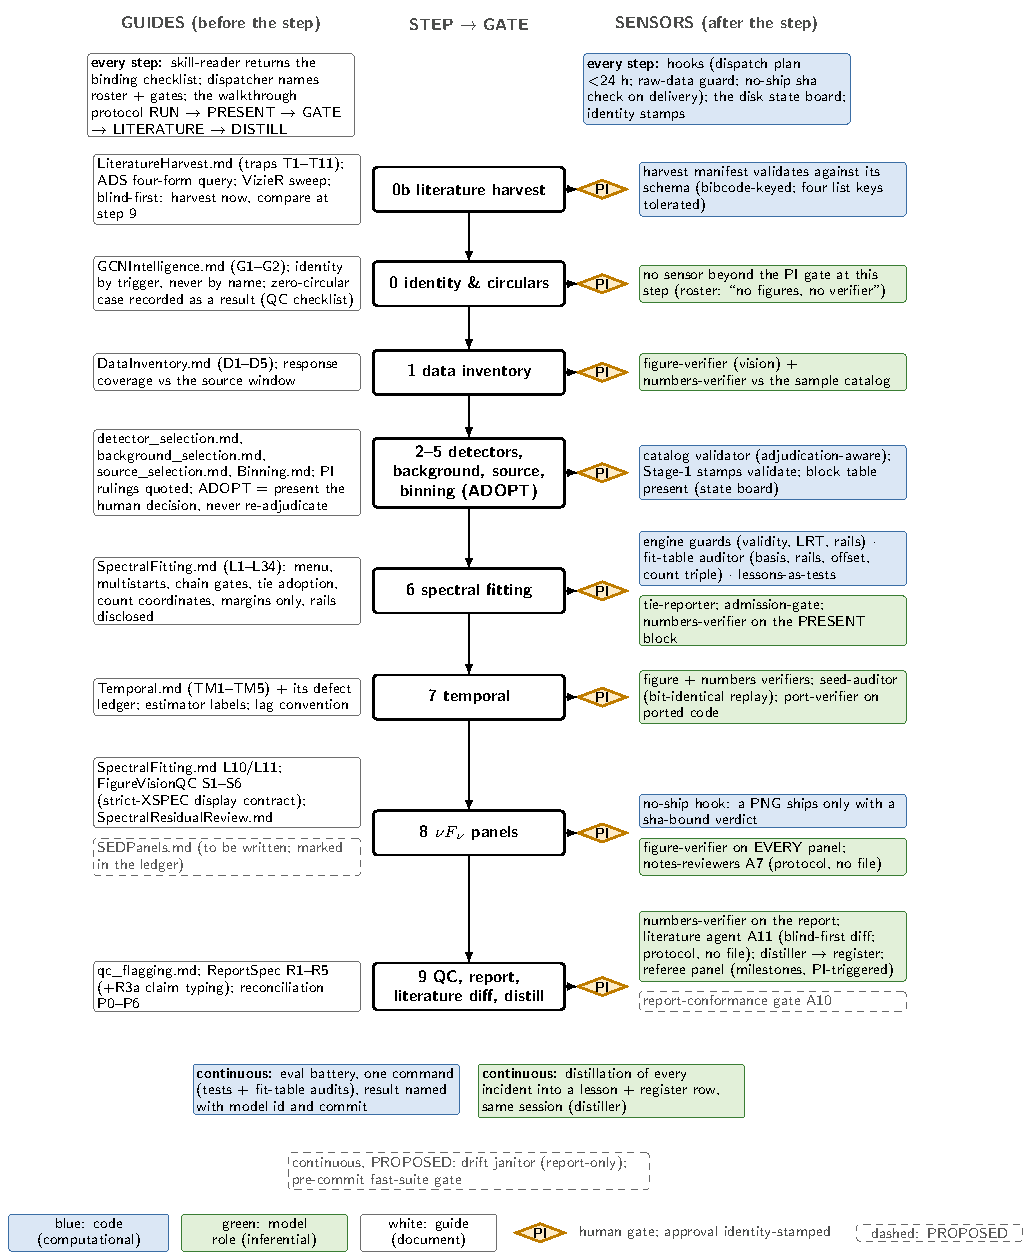
\includegraphics[width=0.92\textwidth]{figures/fig_F2_lifecycle_guides_sensors.pdf}
\caption{The per-burst lifecycle with its guides and sensors. Centre: the
eleven ledger steps, top to bottom, each followed by the human gate.
Left: the guides that steer each step before it runs, chiefly the step's
skill document with its numbered lessons and the standing contracts in the
human's words. Right: the sensors that check each step after it runs, grey
where the check is code (tests, hooks, the fit-table auditor, schema
validation) and white where it is a fresh-context role (figure, numbers,
seed, port verifiers; the tie reporter; the admission gate). Below the
ledger, the checks that run continuously. Dashed items are proposed.}
\label{fig:lifecycle}
\end{figure*}

\subsection{The eleven steps} \label{sec:steps}

The ledger begins before the data. The \emph{literature harvest} (step 0b)
finds and fetches every refereed paper that analysed the burst, using at
least four query forms (the GRB name, the trigger name, the day fraction, the trigger
number), preferring the version of record, and recording each harvested
value with its conventions: which peak-energy definition, which sign
convention for the lag, which energy band, which time interval on whose
clock, which detectors. The harvest is taken early and compared late; the
comparison itself waits for step 9, after our own numbers are frozen
(\S\ref{sec:doctrine}). The \emph{identity and circulars} step (0)
resolves which burst this actually is, since same-day triggers exist, and
reads every real-time circular; a burst with no circular is recorded as a
result, not as a gap. The \emph{data inventory} (1) verifies that the
downloaded data can support the analysis: file versions, response-matrix
time coverage against the source window, and detector geometry, including
the check that no well-placed detector is occulted by the spacecraft, a
failure invisible to pointing angles alone. The three \emph{selection}
steps (2--4: detectors, background windows, source window) are decided by a
human in a purpose-built interface or by a vision-capable role, and either
way recorded with a stamp naming the decision-maker and the mode; downstream
the pipeline treats those stamps as immutable inputs, and the walkthrough
presents the recorded decision rather than re-adjudicating it. The
\emph{adaptive binning} step (5) derives Bayesian-block time bins from the
reference detector and merges them to a significance floor. \emph{Spectral
fitting} (6), where most of the bounded agency lives, has its own
subsection below. The \emph{temporal} step (7) measures the duration, the
minimum variability timescale, and the spectral lag from the same approved
selections, with the estimator named on every value and the lag sign
convention stated. The \emph{spectral-energy panels} (8) render every bin
under the display semantics of the standard X-ray fitting package and are
read residual by residual. \emph{Quality control} (9) assembles the report,
runs the literature comparison, and closes the burst with a typed verdict
and named flags. A bin in which no model passes the validity gate is
declared inconclusive by the engine, and a burst whose response does not
cover its source window is excluded structurally; both are recorded,
\emph{successful} outcomes. The workflow is forbidden to keep adjusting an
analysis until it manufactures a preference.

The guides are the same kind of object at every step: the step's skill
document, read end to end by the skill reader before the step opens, with
its criteria, its checklist, and, where the step has accumulated them, its
numbered lessons; for the selection
steps the human's rulings quoted verbatim; for the figure and report steps
the standing contracts. The sensors differ by step because the artifacts
differ. A harvest manifest is validated against its schema. An inventory
figure passes the figure verifier and its numbers are recomputed against
the sample catalog. A stamped selection is validated by the catalog
validator, and the state board records the block table before fitting may
start. A fit table passes the engine's own guards, the fit-table auditor
(the argmin, the rails, the tie set, the count coordinates), the
lessons-as-tests, and, on presentation, the tie reporter and the numbers
verifier. A temporal product passes the figure and numbers verifiers, the
seed auditor, which replays any stochastic product from its recorded seed,
and the port verifier where code was ported. A panel cannot reach the human
unless its hash is in the verification ledger, and every panel is read by
the figure verifier. The report passes the numbers verifier and the
blind-first literature comparison; a report-conformance gate that would
check the report against its contract as code is specified and proposed.
Beneath the ledger two checks run continuously: the evaluation battery,
one command that runs the test suite and the fit-table auditor over every
promoted table and records, with its result, the model identity it was
given and the commit,
and the distillation of every incident into a lesson and a register row
in the session that produced it (\S\ref{sec:learning}).

\subsection{Inside the fitting step} \label{sec:fitstep}

The fitting engine confronts each time bin with twenty-four spectral
models: six base models, two free-smoothness variants, and sixteen
high-energy extensions (Fig.~\ref{fig:fitstep}). Three rules govern what
the numbers may mean. First, \emph{inclusion is gated on data quality,
never on detection significance}: every detector band with usable data and
a valid response enters the joint fit, because conditioning inclusion on
significance manufactures spurious detections in exactly the bursts where a
band fluctuated upward. Second, \emph{every model family receives multistarts}: unconditional for
the continua and the two-break family, and triggered for the thermal
composites whenever the thermal component rails or fails its nested test,
because a chained seed from a bright epoch can strand a faint bin in a
wrong local minimum, a failure we document in \S\ref{sec:learning}. Third, \emph{validity gates} exclude from model
selection any fit whose shape parameters sit on a bound, with the margins
computed in the parameter's natural geometry (logarithmic for energy-like
parameters spanning decades), a rule the campaign learned from its first
soft burst.

\begin{figure*}[t]
\centering
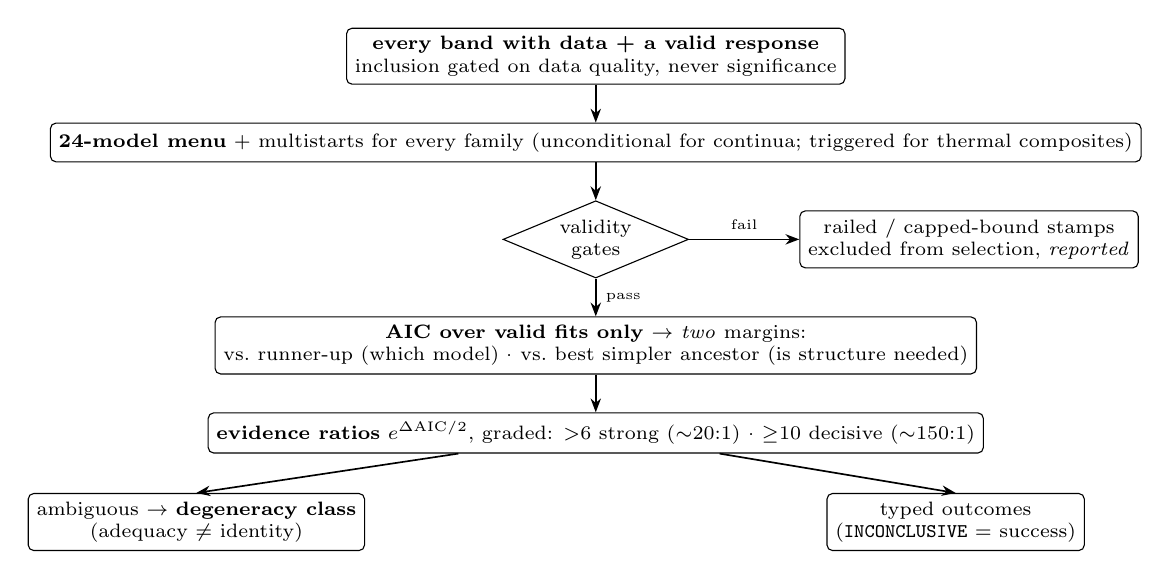
\begin{tikzpicture}[node distance=4.8mm and 7mm]
\node[box] (data) {\textbf{every band with data + a valid response}\\inclusion gated on data quality, never significance};
\node[box, below=of data] (menu) {\textbf{24-model menu} + multistarts for every family (unconditional for continua; triggered for thermal composites)};
\node[dec, below=of menu] (valid) {validity\\gates};
\node[box, right=14mm of valid] (excl) {railed / capped-bound stamps\\excluded from selection, \emph{reported}};
\node[box, below=of valid] (aic) {\textbf{AIC over valid fits only} $\rightarrow$ \emph{two} margins:\\vs.\ runner-up (which model) · vs.\ best simpler ancestor (is structure needed)};
\node[box, below=of aic] (ev) {\textbf{evidence ratios} $e^{\Delta\mathrm{AIC}/2}$, graded: $>$6 strong ($\sim$20:1) · $\geq$10 decisive ($\sim$150:1)};
\node[box, below left=5mm and -20mm of ev] (deg) {ambiguous $\rightarrow$ \textbf{degeneracy class}\\(adequacy $\neq$ identity)};
\node[box, below right=5mm and -20mm of ev] (ok) {typed outcomes\\(\texttt{INCONCLUSIVE} = success)};
\draw[arr] (data)--(menu); \draw[arr] (menu)--(valid);
\draw[arr] (valid)-- node[lab, above]{fail} (excl);
\draw[arr] (valid)-- node[lab, right]{pass} (aic);
\draw[arr] (aic)--(ev); \draw[arr] (ev)--(deg.north); \draw[arr] (ev)--(ok.north);
\end{tikzpicture}
\caption{Inside the fitting step. The engine is deterministic; the agent's
bounded agency is the audited interpretation of its outputs.}
\label{fig:fitstep}
\end{figure*}

Model comparison is then reported as evidence, not verdicts. The engine
ranks the valid fits by the Akaike information criterion and writes the
winner; the interpretation quotes the winner's margin twice, against the
runner-up (\emph{which} model) and against the best simpler model it nests
(\emph{is the extra component needed at all}), each converted to an
evidence ratio $e^{\Delta\mathrm{AIC}/2}$ and graded. A margin above 6
corresponds to more than roughly 20:1 and is tracked as strong; at or
above 10, roughly 150:1, decisive; anything less is reported as what it
is. Heads within two units
of each other are a tie, never a winner: the tie is reported as a set, and
where one model must be adopted for a downstream product the adoption rule
prefers the fewest parameters and then the lowest criterion, and says so.
Where extra structure is required but thermal and non-thermal descriptions
sit within a few units of each other, the bin is assigned to a degeneracy
class rather than a physics claim: \emph{adequacy and identity are
different questions}, and the second frequently cannot be answered from
these data alone. Two further stamps ride on the artifact rather than in prose: a
bound-pinned parameter is flagged on the fit row where it sits, and the
audit record beside the table classes every thermal component by where
its peak, at $3.92\,kT$, falls: below the detector band, inside it but
below the 20~keV trust floor (edge-constrained), marginal, or in band, so
that a reader of the table sees the condition without reading the report.

\subsection{Fan-out and the gates} \label{sec:fanout}

Producers fan out: the fitting engine over time bins, the panel builders
over models, the harvest readers over the published literature. Their
outputs converge on verifier gates, each a fresh-context role with one
duty (Table~\ref{tab:roster}). Every figure passes a vision check before
any human sees it. Every printed number is recomputed from the run's own
products. A model-selection margin below the tie threshold is reported as
a tie. A stochastic product must rerun bit-identically from its recorded
seed. A ported algorithm is compared numerically with its source before it
is trusted. No row enters a committed catalog unscreened. Nothing is
re-derived that the project has already proven. Every incident is closed
into a lesson, at the correct enforcement layer, in the same session that
produced it. A verdict is bound to a content hash of the artifact it
certifies and expires the moment that artifact changes. The assembly is the
reverse of the fan-out: verified outputs are composed into the burst's
report, the burst's typed state advances only when the products on disk
evidence it, and the human's approval of step 9 closes the burst.

Two disciplines that wrap the lifecycle belong to later sections. Before
any comparison with the literature, our own numbers are frozen, and every
mismatch is attributed to our side, to the published side, or to a
difference of frame; that protocol is the verification doctrine of
\S\ref{sec:doctrine}. And the lifecycle's exit condition is convergence:
when $K$ consecutive bursts complete without a new lesson, the skill
library is declared converged, the pipeline is frozen at a recorded commit,
and the whole sample is re-analysed once by the frozen system; that
steering loop is \S\ref{sec:learning}. Only the frozen sweep produces
citable numbers, and every value in this paper from the walkthrough era
carries the provisional flag\prov.


% ---- v3 claims block (decision 20, gate 2): §5 + §6 from fragments; v2 §4-§5 replaced (see
% ---- paper_agentic/v3/DECISION_SHEET_claims_block.md §3 for where every v2 paragraph went).
% ===========================================================================
% v3 §5 — THE STEERING LOOP: LEARNING WITHOUT GRADIENTS (~2 pp; F4, F7, T2)
% Draft r1 (2026-09-03), claims block with §6 and §10 (decision 20). Replaces v2 §4 "Learning Without
% Gradients" (v2:505-609): first two paragraphs and the two episodes kept in substance; the register and
% the enforcement hierarchy (from v2's "operating skeleton") moved here; the id-collision worked example added;
% divergence learning kept; K/freeze stated as the exit rule with "not yet exercised".
% Counts (census 2026-09-03): 43 heading-form numbered lessons in the five step skills that carry them
% (L 31 present of ids to 34, TM 5, D 5, G 2, T 11 — dev/build_learning_curve.py census); register 49 NR
% rows: 20 DEPLOYED, 21 PROPOSED, 3 PARTIAL, 5 closed/practice/fix-applied; 9 rows with a keep: clause.
% Figure F4 = figures/fig_F4_steering_loop (gated); F7 = figures/fig_F7_learning_curve (dev/build_learning_curve.py).
% Decisions 18/19: describe what runs; no claims. \cite keys are v2's (in agentic_grb.bib).
% ===========================================================================
\providecommand{\rc}[1]{\parbox[t]{10.2cm}{\raggedright #1}}   % register-table cell; move to the preamble at splice
\section{The Steering Loop: Learning Without Gradients} \label{sec:learning}

Contemporary AI agents are improved in five ways: pretraining on large
corpora; supervised fine-tuning on demonstration trajectories; preference
optimization against human or model judgments; reinforcement learning on
\emph{verifiable} rewards, where a trajectory is reinforced only if its
outcome can be checked mechanically; and \emph{harness-side learning}, in
which the model's weights are never touched and the surrounding harness,
its instructions, procedures, and memory, accumulates capability instead
\citep{2025Natur.645..633G,2023arXiv230516291W,2023arXiv230311366S}. Our
campaign is training of the fifth kind carrying the fourth kind's essential
ingredient. The weights of every model we use are frozen; the artifact that
learns is the skill library; and the unit of learning is constrained to be
verifiable: a lesson enters the library only as a claim with provenance
(which burst, which date, which evidence) together with an executable test
that fails if the lesson is ever violated again. The suite runs against the
current analysis products; where a table predates a fix, the failure is
registered in a known-stale ledger with its clearing condition rather than
silenced. Debt is visible, never normalized.

Figure~\ref{fig:steering} draws the loop that produces the lessons. An
\emph{incident} is a defect caught by anyone: a verifier, a test, the
external auditor, or the human at a gate. A \emph{prior-art reader} asks
first whether the project has already proven the point, because
re-deriving a known result is the campaign's most expensive habit. The
\emph{distiller}, in the same session that saw the incident, drives the
root cause to the primitive and chooses the strongest enforcement layer
that can hold the countermeasure: code over hook over artifact over agent
over prose. A rule that can be a test becomes a test; a rule that can only
be a sentence in a skill file is written as one and marked as the weakest
layer. The countermeasure is then recorded twice: as a numbered lesson in
the step's skill file, and as a row of the requirements register that
names the incident that bore it, the layer chosen, and whether the guard is
deployed or proposed. Nine rows so far carry a \emph{keep} condition, the
observable that would show the guard no longer holds. The loop closes on
the next burst, which runs a better pipeline.

\begin{figure*}[t]
\centering
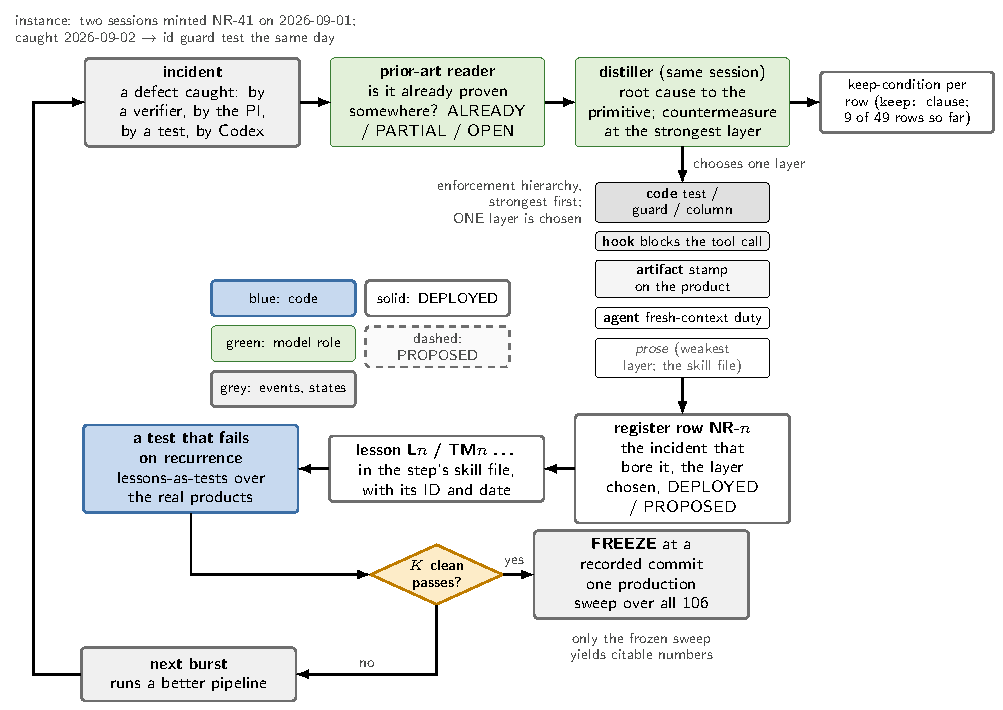
\includegraphics[width=0.95\textwidth]{figures/fig_F4_steering_loop.pdf}
\caption{The steering loop. An incident, caught by a verifier, a test, the
external auditor, or the human, passes a prior-art reader and a distiller
(green: model roles) that place the countermeasure at the strongest layer
of the enforcement ladder (grey rungs, graded by strength), then record it
as a register row and a numbered lesson (white: documents) with a test that
fails on recurrence (blue: code). The amber diamond is the human's decision
to declare convergence after $K$ clean passes; the freeze and the single
production sweep follow. Neither has yet occurred: $K$ is not set and no
clean pass has been recorded.}
\label{fig:steering}
\end{figure*}

This training style has properties that gradient methods cannot offer at
our scale, and one property they share. It is data-efficient: the five
step skills that carry lessons hold forty-three numbered lessons\prov,
twenty-seven of them attributed to the nine bursts walked so far and the
rest to the campaign batches between walkthroughs. It is auditable: the learned policy is plain
text, and every rule cites the burst that paid for it. It transfers across
model families: the same library is executed by different vendors' agents,
which is the basis of the multi-system comparison of \S\ref{sec:design}.
It survives model upgrades. And, the shared property, it exhibits a
learning curve (Fig.~\ref{fig:curve}), whose flattening is the campaign's
stopping criterion: when $K$ consecutive bursts produce no new lesson, the
library is declared converged, the pipeline is frozen at a recorded commit,
and the whole sample is re-analysed once by the frozen system. Only that
sweep produces citable numbers.

\begin{figure}[t]
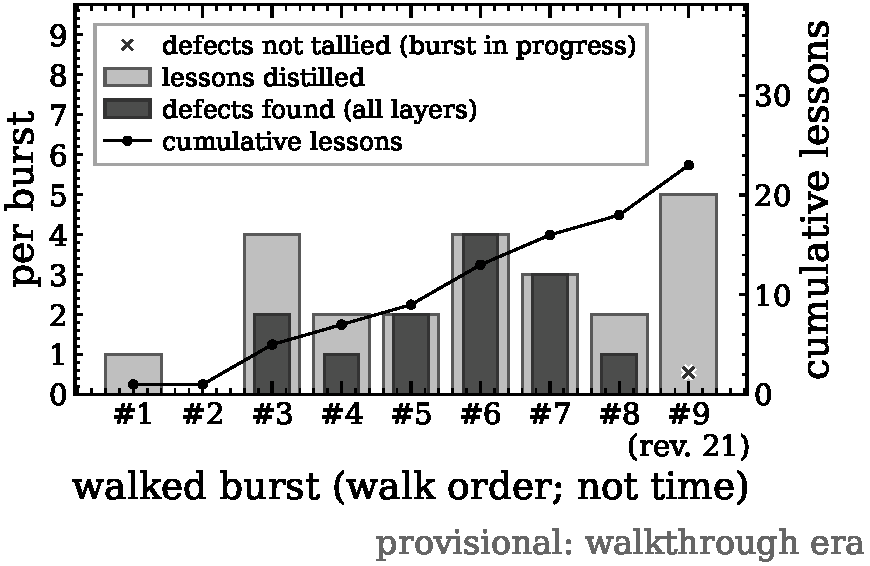
\includegraphics[width=\columnwidth]{figures/fig_F7_learning_curve.pdf}
\caption{The campaign learning curve\prov: lessons distilled per walked
burst (bars), engine defects found (dark bars), and the cumulative lesson
count (line), from the campaign ledger for the first eight walked bursts
and from the dated lesson entries for the walkthrough burst still in
progress. The curve is visibly unconverged; its flattening, not a preset
burst count, terminates the training phase.}
\label{fig:curve}
\end{figure}

\subsection{The register} \label{sec:register}

The register is the campaign's institutional memory: forty-nine numbered
rows\prov, one per needed guard or agent, each carrying the incident that
revealed the need, the layer chosen, and the status. Table~\ref{tab:register}
summarises it and shows eight rows in full. Twenty rows are deployed,
twenty-one are proposed, three are partial (the sensor side built, the
producer side not), and five are closed or recorded as practice. The
dispatcher reads the register at every task intake, so a missing guard is a
stated liability rather than a silent gap, and the register's own rule
applies to itself: a row is minted in the session that saw the incident,
and a proposed guard is listed as proposed until code or a file exists.

\begin{deluxetable*}{lll}   % aastex deluxetable rejects p{} columns; wrapped cells via \rc
\tabletypesize{\footnotesize}
\tablecaption{The requirements register: summary and eight rows in full (census 2026-09-03).\label{tab:register}}
\tablehead{\colhead{row} & \colhead{purpose (the incident that bore it)} & \colhead{status}}
\startdata
\multicolumn{3}{l}{\textit{summary: 49 rows; 20 deployed, 21 proposed, 3 partial, 5 closed or practice; 9 with a keep condition}} \\
NR-1 & \rc{band-validity guard: containment and railed-fraction checks before any spectral band ships (the montage that contradicted its own engine table)} & deployed, code \\
NR-19 & \rc{invalidation cascade: an amended approval clears downstream markers and demotes later approvals mechanically} & deployed, code \\
NR-22 & \rc{skip-by-existence is not skip-by-currency: a marker certifies that a product exists, not which inputs built it} & proposed \\
NR-24 & \rc{report-conformance gate: an assembled deliverable verified against the report contract, including hash equality of report, figures, and table} & proposed \\
NR-30 & \rc{dispatch-hook coverage: the hook that requires a dispatch plan covers one of five launch paths} & proposed \\
NR-44 & \rc{margins-only reporting: information-criterion differences, never absolute values, on this engine} & deployed, code \\
NR-47 & \rc{two-hat separation: the external auditor is never supervisor and blind referee on the same product version} & deployed, protocol and machinery \\
NR-48 & \rc{derived columns recomputed on cell replacement: a promoted table's stored winner must equal the validity-gated argmin over all model columns} & partial (sensor deployed, promotion path proposed) \\
\enddata
\end{deluxetable*}

\subsection{Three episodes} \label{sec:episodes}

Three episodes show what the loop learns and how. The first is a defect we
designate L27. The engine's validity gates flagged a fitted parameter as
railed when it sat within a fixed \emph{linear} margin of its bound. For
energy-like parameters bounded across three decades, that linear margin is
an absolute dead zone of tens of keV above the lower bound, and every burst
analysed in the campaign's first seven walkthroughs had a peak energy far
above it. The eighth burst was soft ($\Ep\sim50$--140~keV\prov), and the
gate silently disqualified every one-break continuum in most of its time
bins, delivering the blocks to thermal-composite models by forfeit.
Uncorrected, the census would have manufactured a population-level
correlation between spectral softness and thermal components, a selection
bias in the costume of physics. The repair (margins computed in the
parameter's natural geometry), its unit test, and the burst's refit
happened within the same session; the pre/post contrast, most blocks
``preferring'' extra structure before and none after\prov, is the measured
size of the bias the lesson prevents. The episode is also an argument about
curricula: the defect was invisible until the sample's serial ordering
happened to deliver a soft burst, so regime coverage, not burst count, is
what a training sample must supply.

The second episode is a cross-validation. Our temporal chain carried a
known, ledgered defect: a spectral-lag sign convention inverted with respect
to the field's standard. The eighth burst has a published lag of
$+7.08\pm0.45$~s in the conventional sign \citep{2018ApJ...865..153L}; our
chain returned $-5.99$~s\prov. Same burst, same physical direction, opposite
sign: the ledgered inversion was confirmed against external ground truth in
the course of ordinary operations, and the lesson (state the convention
with every quoted lag; validate the sign against a burst with a published
direction) was distilled with the defect still unfixed at source. The
library records what is \emph{known}, including known-broken.

The third episode is about the loop itself. On 2026 September~1 two
sessions working the same repository each minted a register row numbered
NR-41, for two different guards. The collision was caught the next day when
the building session inventoried the register, and it was closed the same
day at the strongest feasible layer: one row was renumbered, and a test
that fails on any duplicate identifier entered the suite. The same test now
guards the lesson prefixes of every skill file. The incident cost nothing
scientifically and everything procedurally: a register that can hold two
truths under one number cannot be the campaign's memory, and the fix is a
sentence nobody has to remember.

\subsection{Divergence learning} \label{sec:divergence}

Failures are not the only teacher. Where the human's decision and the
agent's proposal diverge and both are defensible, the divergence itself is
the signal, and it is processed under a fixed protocol: detect it; elicit
the human's reason \emph{in their own words} (a guessed rationale is
forbidden; if the human cannot recall, the record says so); validate the
stated reason against the primitives; generalise it only through a
measured census over the sample, never from the single case; and enter it
in a divergence ledger. The founding case is a detector-selection
divergence: the written geometric rule and two independent agent passes
selected seven detectors\prov; the human had selected four\prov. The human's
recollected reason, keep the detectors that triggered the instrument plus
the companion detector on the same spacecraft side, validated exactly
against the mission's trigger record, and reproduces the detector choice of
every published analysis of that burst we harvested. A census of the full
sample\prov{} then measured how much of expert practice that candidate rule
explains: about eighty percent\prov, with the remainder requiring judgment
the written rule does not capture. The written selection rule therefore
stands unamended, and the divergence is recorded as a measurement of
practice, not promoted to a decision rule. The same census exposed a
contract gap: none of the 105 human selection records\prov{} carried a
contemporaneous reason; the single filled record is a retroactive
reconstruction and is stamped as such. Rationale capture at decision time
is now a registered requirement, while the historical blanks stay blank. A
reconstructed reason is never a contemporaneous record. The ledger gives
the paper's closing question its instrument: the convergence rate, how
often the agent's proposal already matches the human's decision, is the
measurable readiness criterion for ever moving a human gate to an
independent approver.


% ===========================================================================
% v3 §6 — VERIFICATION DOCTRINE (~2 pp) — v2 §5 kept (v2:610-684) with three additions: the frozen-prediction
% and attribution rule moved here from v2 §3 (the outline's split); the known-results battery stated at its
% true status (specified, replay not built; the eval battery runs tests + auditor); the referee loop (two hats,
% three blind referees, NR-47) added as machinery — built 2026-09-01, first firing reserved for the finished
% manuscript; and this paper's own §3 supervisor review as the instance (notes/CODEX_REVIEW_paper_v3_sec3_20260902.md).
% Labels: sec:verify (v2) + sec:doctrine (referenced by §3/§4/§7). Decisions 18/19: describe; no claims.
% ===========================================================================
\section{Verification Doctrine} \label{sec:verify}\label{sec:doctrine}

Two disciplines wrap every burst. Before any comparison with the
literature, the agent's own results are frozen, written to the burst's
record in a form that cannot be revised, together with predictions derived
from the harvested literature. Only then are the two compared, and every
mismatch is pushed to one of three attributions: \emph{we-wrong} (an error
on our side, which must be fixed and tested), \emph{they-wrong} (a
documented problem in the published analysis, stated with evidence), or
\emph{frame-difference} (both analyses defensible; the difference traced to
conventions, data selections, or eras, and recorded as a normalisation
rule). The attribution, not the mismatch, is the product: it becomes a
numbered lesson in the skill library, shipped with its test
(\S\ref{sec:learning}).

\subsection{Blind-first analysis with frozen predictions}

Before each burst is fitted, the literature harvest yields a set of
falsifiable predictions, derived from published analyses and never from
our own outputs, which are frozen alongside a commitment that the fit will
not be steered toward them. The comparison happens only after both sides
are immutable. The campaign's scorecards make the point better than
argument. For the eighth burst, the literature predicted a positive
low-energy photon index early in the burst; our blind fit, with independent
binning and a far larger model menu, reproduced it ($\alpha$ up to
$+0.6$\prov). It predicted monotonic hard-to-soft evolution; our blind
$\Ep$ track declined monotonically\prov. But the natural corollary, that a
spectrum this hard should demand a thermal component, was \emph{refuted}:
with the L27-repaired gates, no time bin required extra structure at even
the strong evidence grade\prov. A framework that can refute its own frozen
expectation is demonstrating the property that matters; confirmation alone
demonstrates nothing.

Beyond per-burst predictions, the doctrine specifies a battery of
\emph{known results} against which each burst's record closes: published
spectral-lag values with their sign conventions, published Bayesian-block
edges, published variability-timescale limits, low-energy photon-index
tracks, and, where an instrument we do not fit has published one,
polarization constraints entered as external predictions. Today the
evaluation battery runs the lesson tests and the fit-table auditor over
every promoted table in one command and records the model identity and
commit with its result; the known-results replay is specified and listed
as proposed. Agreement validates the chain that produced our number,
disagreement is pushed through the attribution above, and either outcome
is banked in the record.

\subsection{Independence lives at the primitive}

Twice in the campaign, two analyses agreed closely and both were wrong or
both unnecessary: our fitted blackbody temperature agreed with a published
value to five percent while both components were statistically unrequired;
and in the experiment below, two independent review channels built the
same load-bearing argument on the same silently symmetric
parameterization, corroborating each other into a void conclusion. We
therefore state the doctrine as: \emph{agreement between two analyses is
evidence only in proportion to the depth of the primitives they do not
share}: minimizer, table, column, response model, prior document. $N$
agents reading the same inputs are one opinion wearing $N$ hats. The
fresh-context roles of \S\ref{sec:context} are correlated error-detection
channels under this rule, not independent reviewers; independence is
claimed only for a check that uses a disjoint primitive, source,
implementation, or human.

\subsection{The four-channel experiment: generators, not adjudicators}

We tested whether a panel of AI reviewers could adjudicate a genuinely
contested scientific question, a burst for which two published analyses of
nearly the same data disagree about a thermal component. Four reviewer
channels examined disjoint evidence primitives: the spectral-panel
\emph{images} only; the numeric \emph{fit tables} only; the block-to-block
\emph{evolution tracks} only; and an \emph{adversary} with full access,
briefed to refute the component honestly and permitted to run its own
diagnostic refits. A separately briefed adjudicator then audited all four.

The outcome was double-edged. As \emph{generators}, the channels were
excellent: the image channel found a figure-construction defect invisible
in any table; the adversary localised a cross-normalisation anomaly that we
later identified, via the published literature, as a physically occulted
detector, and demoted a ``decisive'' margin to an artifact of a railed
reference model, both findings surviving audit and entering the engine as
permanent stamps. As \emph{adjudicators}, the channels failed exactly as
the doctrine predicts: the two numeric channels derived identical margin
ladders and returned opposite verdicts (the disagreement was doctrinal, not
evidential); the panel's one unanimous conclusion was traceable verbatim to
a rule in the shared skill library, prescribed unanimity rather than
measurement; and one channel confabulated statistics that do not appear in
its own assigned figure, caught only because the adjudicator reopened the
figure. Two corollaries entered the doctrine. First, \emph{verify the
adversary too}: the adversary claimed a nondeterministic fitting step; five
identical reruns showed spread exactly zero\prov; its variance had been its
own varying invocations. Second, with/without-data refits are attribution
diagnostics only; a data-dropped fit is never evidence for a claim.

\subsection{The referee loop} \label{sec:referee}

The external auditor wears two hats and never both on one product version.
As \emph{supervisor} it reads everything: the brief pins facts by hash,
declares the conventions that could look like defects, lists the claims to
verify, and closes with a question the brief did not ask. As \emph{blind
referee} it reads only what a journal referee reads: the manuscript and its
data statement, with no internal documents, no claims list, and no sight of
the other referees' reports. The panel is three separate invocations with
fixed temperaments, constructive, standard, and adversarial, reviewing
independently in the first round; the response is one deduplicated letter
with demonstrations rather than assurances; a delta round re-fires only the
referees whose points remain open; the loop is capped at two rounds, and
the human is the editor. Convergence is declared by demonstration, never
by agreement. The machinery exists and the supervisor hat has run on this
manuscript's architecture section: it flagged twenty sentences as stronger
than the evidence on disk, eighteen survived our check at the primitive,
and all were rewritten before the section reached the human. The blind
panel is reserved for the finished manuscript, on a version the supervisor
has not seen.


% ===========================================================================
% v3 §7 — THE OBJECT-AND-ACTION MODEL (NEW; ~1 pp; figure F5)
% Draft r2 (2026-09-03): numbers-verifier fixes — ten schemas = nine object types + the approvals file; quarantine
% writes a manifest; invalidate records which step changed.
% Draft r1 (2026-09-03), architecture block with §3 r4 and §4 (decision 20: one gate for §3+§4+§7).
% Tone per decision 18: describe what is typed and linked on disk and which actions are first-class;
% PROPOSED parts named once, no defect chronicle. Decision 19: description of a design, no claims.
% Census: working tree 2026-09-02, tracked code 4df6884; schemas dev/schemas/ (10); roster rows 18–24.
% Figure F5 = paper_agentic/figures/fig_F5_object_action_model (gated; shas in figures/GATE_LEDGER.md).
% The ontology and provenance citations (Gruber 1993; W3C PROV-DM) enter only after their PDFs are local
% (notes/RELATED_WORK_candidates_20260903.md); the text below stands without them.
% ===========================================================================
\section{The Object-and-Action Model} \label{sec:objects}

A long campaign accumulates objects: selections, block tables, fit tables,
panels, reports, and the records about them. The harness of
\S\ref{sec:harness} works only if those objects are typed, if the links
between them are declared rather than remembered, and if the operations
that change them leave a record. Figure~\ref{fig:objects} draws the model
as it exists on disk, in four parts: the objects, the links between them,
the actions that create or change them, and the roles allowed to act.

\begin{figure*}[t]
\centering
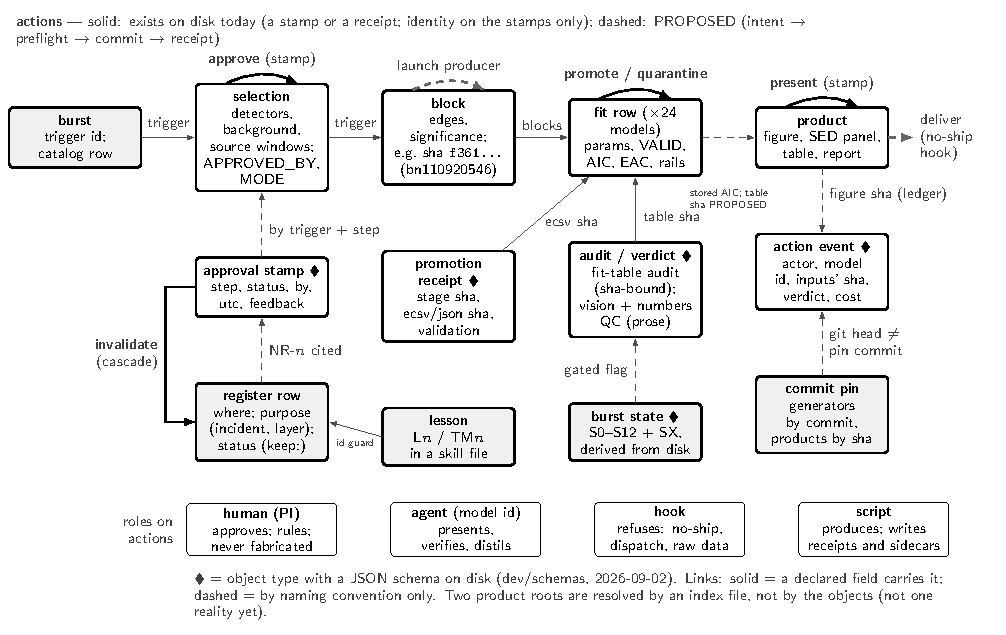
\includegraphics[width=\textwidth]{figures/fig_F5_object_action_model.pdf}
\caption{The object-and-action model. Top row: the burst's chain of
products, from trigger to report. Middle row: the records about those
products. Bottom row: the law that governs them. A diamond marks an object
type with a JSON schema on disk. Links are solid where a declared field
carries them (a trigger key, a content hash, a commit) and dashed where they
hold by naming convention. Actions are labelled arrows, solid where they
are first-class on disk today and dashed where proposed. The band beneath
names the four roles that act. Every box maps to rows of
Table~\ref{tab:roster}.}
\label{fig:objects}
\end{figure*}

\paragraph{Objects.} Thirteen object types are drawn. Five form the
burst's own chain: the \emph{burst} (trigger identifier and catalog row),
the \emph{selection} (detectors, background and source windows, with the
approver and mode stamped on it), the \emph{block table} (bin edges and
significances), the \emph{fit row} (one per model per bin: parameters,
validity flag, information criteria, effective-area corrections, rail
diagnostics), and the \emph{product} (figure, spectral-energy panel, table,
or report). Four are records about products: the \emph{approval stamp}
(step, status, approver, time, feedback), the \emph{promotion receipt}
(hashes of the staged and promoted tables and the validation that passed),
the \emph{audit or verdict} (the fit-table audit bound to the table's hash;
the vision and numbers verdicts), and the \emph{action event} (actor, model
identity, input hashes, verdict, cost). Three are the law: the
\emph{register row} (where a guard lives, the incident that bore it, its
status and keep-condition), the \emph{lesson} (a numbered entry in a skill
file), and the \emph{burst state} (one of the fourteen states of
\S\ref{sec:loop}, derived from disk), together with the \emph{commit pin}
that fixes generators by commit and products by hash. Ten JSON
schemas\prov{} cover nine object types and the per-burst approvals file
that holds the stamps; five of the thirteen drawn here are among them (the
stamp, the receipt, the audit, the action event, and the burst state), and
the others are the literature-harvest manifest and its paper records, the
frozen prediction record of \S\ref{sec:doctrine}, and the fit sidecar. The test suite validates every
instance on disk against its schema. Schemas came late: the pipeline had written
these objects for months before their shape was declared, and the first
validation pass found four spellings of one key in the literature-harvest
manifests. A schema written before the first instance would have cost less.

\paragraph{Links.} A link is declared when a field of one object names
another: the trigger key that ties a selection to its burst and a block
table to its selection; the block indices that tie fit rows to blocks; the
table hash that ties a receipt and an audit to the fit table they certify;
the lesson identifier that a register row cites, guarded by a test that
refuses duplicate identifiers. Links that hold only by convention are drawn
dashed: a stamp finds its selection by trigger and step number, a product
finds its fit rows through the stored information criteria rather than a
recorded hash, a burst state points to the verdicts it summarises by a
flag, and the commit pin relates to the action trace only through the git
head each event records. The distinction matters operationally. A declared
link can be checked by code; a conventional link can only be checked by a
reader who knows the convention. Declaring the remaining links, chiefly the
fit-table hash on every product, is the smallest step that would let the
report-conformance gate of Table~\ref{tab:roster} be written as code.

\paragraph{Actions.} An action is an operation that changes what the
campaign may claim. Four are first-class on disk today, each leaving a
typed record with an identity: \emph{approve} writes a stamp; \emph{present}
writes a stamp; \emph{promote} writes a receipt and \emph{quarantine} a manifest; and
\emph{invalidate} demotes the approvals downstream of an amended step and
records which step changed. Two are proposed and drawn dashed. \emph{Launch producer}
would wrap every pipeline run as intent, preflight, commit, and receipt,
so that a producer could not start without the plan and could not finish
without the sidecar; today the dispatch hook of \S\ref{sec:boundaries}
enforces the first half for the transitions it covers. \emph{Deliver} would
record every artifact handed to the human; today the no-ship hook refuses
an unverified figure but writes no record of what it allowed. The action
trace that would hold all six is on disk with its schema, appended by
protocol; automatic capture of every tool call is the boundary item listed
in Table~\ref{tab:roster}.

\paragraph{Roles.} Four kinds of actor appear on actions, and the model
fixes what each may do. The \emph{human} approves and rules, and no
approval is ever written on the human's behalf. The \emph{agent}, stamped
with its model identity, presents, verifies, and distils. The \emph{hook}
refuses. The \emph{script} produces and writes its receipt and sidecar.
The separation of producer, verifier, and approver in
\S\ref{sec:boundaries} is this role band read as a rule.

\paragraph{One reality.} The model has one structural gap, drawn in the
legend rather than hidden: products live in two roots, resolved by an index
file, so the same burst can have a fit table in each. The objects
themselves do not say which is canonical; the index does, and the
promotion receipt certifies the promoted one. Closing the gap means either
a single root or a canonical-table field on the burst object, and it is the
precondition for the state board to derive every one of its fourteen states
from declared links alone. We list it here because the object model, more
than any agent, is what would let a second group run this campaign and
arrive at the same tables.


\section{Experimental Design: Human versus Agent} \label{sec:design}
% ===========================================================================
The benchmark design retains v1's core: a 25-burst subset receives
independent Stage-1 selections from experienced researchers, and agents from
multiple vendors---executing the \emph{same} Skill Library, so that
differences isolate the model rather than the prompt---are scored not on
matching any single expert but on landing within the \emph{spread of the
experts}, decision by decision: detector sets, background windows, source
intervals, model verdicts. Scoring decisions rather than published numbers
is forced on us by the field itself: published analyses of the same burst
disagree, so the literature is a distribution over defensible choices and
cannot serve as an answer key. \PENDING{the multi-system benchmark run; a
second independent expert completes the human spread}

We add two further controls in operations. The walkthrough queue runs in two
lanes---an older-era lane and a recent-era lane (2021--2025)---so that any
skill, constant, or contract that works in one era and fails in the other
is exposed as a cross-era defect rather than absorbed as noise. In
parallel, a human collaborator replicates the analysis with the Stage-1
selections held fixed, isolating the downstream methodology from
selection scatter.

One scoring rule deserves its own statement, because the data forced it.
For decisions with \emph{no answer key}, agreement between arms is a
\emph{concordance} measure and must never be reported as accuracy:
neither arm can be wrong, a divergence is not an error, and any benchmark
number that scores it as one is invalid. Background-interval placement is
the proving case. For one burst that triggered about two minutes\prov{}
after a radiation-belt exit, two equally defensible uncontaminated
baselines imply excesses in the same interval that differ by a factor of
seven\prov{} ($+68$ versus $+481~\mathrm{counts\,s^{-1}}$): the excess is
real while its magnitude is not a measurement, and the published
literature uses this very burst as its showcase that polynomial
background choices can be ambiguous \citep{2020A&A...640A...8B}. The
benchmark therefore separates its dimensions: rule compliance and
downstream impact are truth-bearing and scored; window agreement is
reported as concordance only. The separation expires only if a physical
background model replaces the polynomial one, creating the answer key
that does not currently exist.

% ===========================================================================
\section{Walkthrough-Era Results} \label{sec:results}\label{sec:casestudy}
% ===========================================================================
All numbers in this section are walkthrough-era and provisional\prov;
they will be regenerated by the frozen production sweep. The full
106-burst sample has passed once through the fitting engine, with one
burst excluded for response-matrix time coverage and reported as an
exclusion rather than silently dropped\prov. No cross-burst census
sentence is permitted yet: a ledgered retry debt concentrated in the
multi-break and composite model families must reach a terminal state
first, and per the doctrine that debt is visible in the products, never
normalized away. Among the walked bursts: a burst whose apparent two-break ``decisive''
margin traced to a railed reference model and now carries a capped-bound
stamp; a burst whose published photospheric identification our wider menu
reduces to a forced choice between statistically equivalent thermal and
non-thermal descriptions; a burst in which the fitted low-energy break and
the fitted blackbody peak track each other at the few-percent level across
eleven bins---one spectral feature wearing two model names; the campaign's
first soft burst (the L27 episode), whose positive low-energy slopes are
carried entirely by one-break continua; the campaign's first
intensity-tracking burst, whose blind $\Ep$ track follows the flux and whose
late-time cutoff evolution sits in open, documented tension with a published
constant-$\Gamma$ curvature interpretation; and the field's best-known
polarimetric burst, for which published polarization-angle rotations enter
the frozen predictions as constraints from an instrument we do not fit.
The architecture itself is under a live acceptance test: the entire
law---skills, roster, gates, skeleton---was handed to a fresh session
with no inherited conversational context, on the argument that an
architecture that works only for its authors is not yet an architecture.
In that arm's first burst, the first seven of the eleven gated steps have
passed their human gates with every approval stamped\prov{}---each stamp
carrying its own provenance, including one approval given colloquially and
typed as read-as-approval, and one recorded late, the case below---and the
mechanisms, not the operators' memories, caught what needed catching. The
approval ledger's cascade exposed an approval that existed only in
conversation for seven hours\prov{} and forced it onto the record with
the delay disclosed. The data-inventory contract surfaced a
hundred-millisecond telemetry stall\prov{} invisible to the standard
exposure accounting (its count deficit is cancelled by a buffered
catch-up in the following readout bin), and the repair was accepted only
under a robustness criterion: the chosen background cut is the one whose
fit quality is independent of the binning grid's phase, which otherwise
moves the fit statistic by up to a factor of 2.4\prov. And a background
window found overlapping the approved source window by about thirty-two
seconds\prov{} was measured as a real excess ($\geq\!3.3\sigma$ in every
fit variant\prov), repaired by an explicit human ruling, and its residual
tail contamination carried forward as a disclosed systematic rather than
silently accepted. Each catch was typed to its failure class and
distilled; the steps beyond the stamped gates remain open and contribute
no accepted numbers here.

The Campaign Ledger records, per burst: lessons born, defects found,
blind-prediction outcomes, and human gate corrections; it is released with
the paper, and Fig.~\ref{fig:curve} is computed from it. External,
zero-cost validations accumulated along the way: our adaptive binning
reproduces a published analysis' Bayesian-block edges to three decimal
places on a shared burst \citep{2021ApJS..253...43L}, and twenty-two of our sample's bursts carry
published lag, width, and evolution-class measurements \citep{2018ApJ...865..153L} against which the
temporal chain is validated burst by burst as the campaign reaches them.

% ===========================================================================
% ---- v3 §10 from the fragment; v2 §8 replaced.
% ===========================================================================
% v3 §10 — DISCUSSION (~2 pp; T4, F8) — v2 §8 (v2:786-864) kept for the failure taxonomy, the capability
% boundary, and "what generalizes"; NEW: the two newest failure modes (the inherited figure string; the
% late stamp), the needs/strengths table T4 from the five-source synthesis (notes/HARNESS_COMPARISON §19/§20,
% statuses at the 2026-09-03 census), the runtime-vs-eval harness figure F8; the creativity outlook shortened
% to one paragraph (its citations kept). F6 (context x action map) DROPPED: it was the posts' framing
% (decision 17: not cited). Decisions 18/19/25: describe; no claims; proposed stays proposed, on hold.
% ===========================================================================
\providecommand{\nc}[2]{\parbox[t]{#1}{\raggedright #2}}   % needs-table cell; move to the preamble at splice
\section{Discussion} \label{sec:discussion}

\subsection{Failure taxonomy} \label{sec:failures}

Every mode below was observed in this campaign, caught, and converted into
doctrine; none was caught by the failing agent itself.
\emph{Over-claiming}: three retracted claims, each computed from technically
correct numbers whose validity flags had not been checked; caught by the
human gate and by an independent agent audit. \emph{Prescribed unanimity}:
a panel's unanimous verdict traced verbatim to the shared prior document
(\S\ref{sec:verify}). \emph{Confabulation}: a reviewer channel reporting
statistics absent from its own assigned figure. \emph{Estimator mismatch}:
an ad hoc quality check using a simpler background model than production,
manufacturing a $5.6\sigma$ alarm against a selection a human had already,
correctly, approved; the rule is that a check must use the production
estimator or it is not a check. \emph{Tool-interface drift}: invoking one's
own tools with invented arguments. \emph{Momentum skips}: advancing past a
presentation step the protocol requires; caught by the human, converted
into an explicit rule. \emph{Diagnostic-becomes-result drift}: treating a
data-dropped sensitivity refit as evidence. Two modes are newer. \emph{The
inherited string}: a figure carried unchanged from one draft to the next
kept a state name that exists nowhere in the repository, and survived
because ``unchanged'' exempted it from the check every sentence gets; the
countermeasure proposed to the distiller is that an inherited figure
string is verified like prose.
\emph{The late stamp}: an approval given in conversation and reported as
recorded was never written to disk, and was found only when the
invalidation cascade looked for a stamp to demote; the record carries it
dated to the conversation with the delay disclosed. The live report is
assembled from the stamps on disk and shows a step as approved only where
a stamp exists; the guard distilled from the incident, stamp on the gate
answer before any other action, is recorded with the stamp and is not yet
a register row. The taxonomy
is the practical answer to ``where does the agent still need a human'': at
every point where the system's own priors, momentum, or plausible but
unchecked numbers are the failure mode, because those are precisely the
failures self-review does not catch.

\subsection{The capability boundary}

The same experiments that expose these failures locate the boundary
positively: differently primed AI reviewers are strong \emph{generators} of
checkable findings, several of which entered the engine as permanent
guards, and weak \emph{adjudicators} of contested verdicts. We therefore
spend agency where generation pays (proposing, localising, refuting,
attributing) and reserve adjudication for the gated human, with the audit
trail as the interface between them.

\subsection{What the harness lacks, and what it has} \label{sec:lacks}

We compared the harness, component by component, with the engineering
accounts of agent harnesses that have appeared since we built it.
Table~\ref{tab:needs} states the result in both directions: what those
accounts ask for that we do not have, with its status at the census, and
what the campaign has that none of them describes. The first column is
mostly a list of mechanisms that would turn protocol into machinery:
structured traces of every action with the model identity on every
product, one evaluation battery run on every harness or model change,
first-class actions with receipts, caps and cost limits on every loop,
computational sensors ahead of inferential ones, a sandbox for producers,
and interception points beyond the one tool-call hook. None of the eight
is complete: four have their artifact built (the trace and stamp modules,
the battery, the schemas) with the remainder held or proposed; two have a
single instance (the referee cap; the four countable auditors); one is
proposed and one is held, by the human's ruling that nothing is built
ahead of a walked burst's need: the campaign is meant to have more than
the essential and not to be over-engineered ahead of evidence. The second
column is the science-specific behaviour harness: blind-first
reconciliation as a method, verdicts bound to the artifact's hash, the
human's words as the contract, the register with its incidents, disk-derived
state with identity-stamped approvals, the blind referee panel, the numbers
discipline, honest limits on every gate, a mechanical no-ship gate, and a
design taken from the bursts walked and from the incidents behind the
register's rows, which name fourteen bursts, rather than from a component
list.

\begin{deluxetable*}{lll}   % aastex deluxetable rejects p{} columns; wrapped cells via \nc
\tabletypesize{\footnotesize}
\tablecaption{What the harness lacks and what it has, from a comparison with five engineering accounts of agent harnesses (census 2026-09-03).\label{tab:needs}}
\tablehead{\colhead{asked for, not (fully) present} & \colhead{status} & \colhead{present here, described in none of them}}
\startdata
\nc{5.1cm}{structured trace per action and per agent invocation} & \nc{3.6cm}{artifact and schema built; automatic capture held} & \nc{7.3cm}{blind-first reconciliation with frozen predictions and three-way attribution} \\
\nc{5.1cm}{model identity on every product; retest on model change} & \nc{3.6cm}{stamp module built; wiring into pinned generators held} & \nc{7.3cm}{verdicts bound to the artifact's hash, expiring on edit, from a fresh-context verifier} \\
\nc{5.1cm}{one evaluation battery on every harness or model change} & \nc{3.6cm}{built (tests + fit-table auditor over every promoted table; known-results replay proposed)} & \nc{7.3cm}{the human's words as the contract: standing items and rulings quoted and dated} \\
\nc{5.1cm}{typed objects, declared links, first-class actions with receipts, roles} & \nc{3.6cm}{ten schemas built; actions and one-reality proposed} & \nc{7.3cm}{the register: every guard carries the incident that bore it; distillation the same session} \\
\nc{5.1cm}{caps and cost limits on every loop} & \nc{3.6cm}{referee loop capped; others proposed} & \nc{7.3cm}{disk-derived state and identity-stamped approvals; a chat-only approval is a defect} \\
\nc{5.1cm}{computational sensors before inferential agents; pre-commit gate; drift janitor} & \nc{3.6cm}{four countable auditors coded; pre-commit and janitor proposed} & \nc{7.3cm}{the two-hat auditor and the three-referee blind panel with fixed temperaments} \\
\nc{5.1cm}{a sandbox for producers} & \nc{3.6cm}{proposed (raw-data hook is the only containment)} & \nc{7.3cm}{the numbers discipline: count coordinates, margins only, rails disclosed, ties as ties} \\
\nc{5.1cm}{interception points beyond one tool-call hook} & \nc{3.6cm}{held (changes a live session's settings)} & \nc{7.3cm}{honest limits stated on every gate; a mechanical no-ship gate at delivery} \\
\enddata
\end{deluxetable*}

\begin{figure}[t]
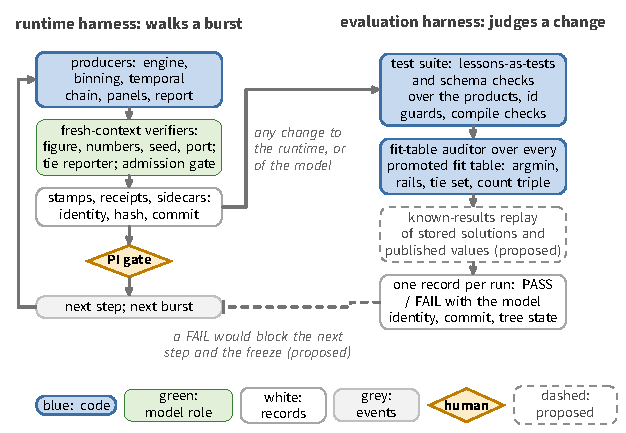
\includegraphics[width=\columnwidth]{figures/fig_F8_eval_harness.pdf}
\caption{Two harnesses. Left, the runtime harness that walks a burst:
producers, fresh-context verifiers, stamps, and the human gate. Right, the
evaluation harness that judges a change to the runtime: the test suite,
the fit-table auditor over every promoted table, and the proposed
known-results replay, run as one command whose record carries the model
identity and the commit (counts at the 2026 September~3 census). Every
change to the runtime harness, and every change of model, is a reason to
run the right-hand side, but that trigger is a discipline rather than a
hook: the pre-commit gate that would enforce it is proposed. The counts are
the census of 2026 September~3, and the promoted tables are those of the
twenty-five bursts promoted so far. The dashed return, a failed battery
blocking the next step and the freeze, is proposed: today the battery
records its verdict and nothing yet consumes it.}
\label{fig:evalharness}
\end{figure}

\subsection{What generalizes}

Gates with stamps, lessons-as-tests, blind-first frozen predictions,
frame alignment before any diff, independence at the primitive, and the
failure taxonomy are domain-agnostic and export as a package; the engine,
the menu, and the lessons' content are the domain deposit that makes the
package worth executing. Both are released. The level at which the package
is designed is the component: the roster of Table~\ref{tab:roster} is the
unit a second group would reproduce, and the science-specific behaviour
harness, the numbers discipline and the blind-first rule, is what a physics
pipeline adds to the generic parts. The skill library, the register, the
role contracts, and the doctrine are text and transfer unchanged across
vendor agent platforms; the enforcement layer, hooks, state derivation,
cascades, is rebuilt per platform. We treat that portability as an
experiment rather than an assumption: the same law executed by a second
vendor's agent on a known burst, compared gate by gate, is the designed
test, and it is pending.

\subsection{Outlook: the discovery plane} \label{sec:creativity}

The production plane described in this paper deliberately excludes
open-ended discovery; a second, sandboxed plane exists for it, governed by
one rule: the agent may invent a new scorecard after seeing the game, but
may not pretend the scorecard was chosen before the game. What would make
that plane generative rather than merely permitted is a hypothesis we are
developing: that creative scientific acts are, predominantly, typed
operations on the knowledge graph of the literature, drawing an edge along
a long or never-co-cited path, negating a named load-bearing assumption of
a published derivation, or constructing a new graph element outright
\citep{boden2004,swanson1986,2013Sci...342..468U,2013arXiv1302.6906F,wiggins2006}.
The reconciliation protocol already extracts, burst by burst, the
assumption-level statements such a graph requires; the discovery plane is
where they would compound. We state it as a direction, not a result.


\section{Conclusions} \label{sec:conclusions}
% ===========================================================================
Yes---as a gated workflow with bounded agency, trained harness-side under
verifiable lessons, and audited by a doctrine that treats agreement with
suspicion and refutation as a service. The system walks bursts end to end
under stamped gates, has taught itself thirty-two durable lessons\prov,
found its own engine defects including one census-grade
selection bias, validated a known defect against published ground truth,
refuted one of its own frozen predictions, and now runs as written in a
fresh session with no inherited context---the acceptance test of
\S\ref{sec:results}. The per-burst numbers are provisional by design; the Skill
Library is not. When the learning curve flattens, the pipeline freezes and
runs the full sample once; that sweep, not this paper, produces the census.
The question in the title has an honest answer only with its architecture
attached---and that architecture, we argue, is the contribution.

We do not mistake the current boundary for a permanent one. Every failure
mode in \S\ref{sec:failures} was caught at a gate, and every catch became a
lesson: the gates are where human judgment is \emph{transferred}, not merely
exercised, and the Library is the accumulating transfer. The claim that some
capability---taste in ambiguous selections, suspicion of one's own
agreement, the adjudication of contested verdicts---is inherently human is,
under this architecture, an empirical claim about the tail of a learning
curve, testable by whether the gate-correction rate falls to zero as
lessons accumulate. The Divergence Ledger of \S\ref{sec:divergence} makes
that test operational: the convergence rate between the agent's proposal
and the human's decision is now a defined, recorded quantity, accumulating
with every gate\prov.
And the curriculum need not stop at analysis: the
discovery-plane operators of \S\ref{sec:creativity}---bridging stale regions
of the literature graph, negating named load-bearing assumptions,
constructing new observables---are mechanisms by which discovery itself
becomes teachable. Whether the gates ever go fully quiet is not something
this paper can assert; it is something this campaign, continued to
convergence and beyond, is built to measure. The gate, in the end, is a
curriculum---and curricula are meant to be completed.

\appendix
\section{Component roster} \label{app:roster}
Table~\ref{tab:roster} lists every component of the harness of \S\ref{sec:harness} with its job in one sentence, its kind, how it executes, and its status at the census.
% T1 — component roster, GENERATED from paper_agentic/T1_component_roster_DRAFT.md (commit 427fdc5) by the build script; do not hand-edit.
\startlongtable
\begin{deluxetable*}{lllll}
\tabletypesize{\footnotesize}
\tablecaption{The component roster: the work of each component in one sentence. Kind: guide / sensor / action / store / producer / actor / boundary; execution: computational (C), inferential (I), human (H). Status is what is on disk at commit \texttt{4df6884} (census 2026-09-02): DEPLOYED = a file or product exists; PROPOSED = a register row or law-file actor without one. Origins are quoted in the source table.\label{tab:roster}}
\tablehead{\colhead{component} & \colhead{job} & \colhead{kind} & \colhead{exec.} & \colhead{status}}
\startdata
\multicolumn{5}{l}{\textit{the loop (run the reasoning loop)}} \\
\parbox[t]{4.0cm}{\raggedright Mode-B harness session (Claude Code plays the roster)} & \parbox[t]{7.2cm}{\raggedright Runs the reasoning loop in a subscription coding harness, consuming the agent files, hooks and skills natively while humans gate in-session.} & \parbox[t]{2.0cm}{\raggedright actor} & I & DEPLOYED \\
\parbox[t]{4.0cm}{\raggedright Burst-walkthrough protocol + fresh-session boot ritual} & \parbox[t]{7.2cm}{\raggedright Opens every session from the law files and the disk board, then presents each of the eleven steps to a gate before the next runs.} & \parbox[t]{2.0cm}{\raggedright guide} & I/H & DEPLOYED \\
\parbox[t]{4.0cm}{\raggedright Dispatcher (A2)} & \parbox[t]{7.2cm}{\raggedright Reads the task and the register, then returns the agents, gates and order required, naming every guard that is still unbuilt.} & \parbox[t]{2.0cm}{\raggedright actor (planner)} & I & DEPLOYED \\
\parbox[t]{4.0cm}{\raggedright Queue manager + workflow set (A17; \texttt{wf-*})} & \parbox[t]{7.2cm}{\raggedright Would own campaign sequencing: read every burst state, run the next legal transition as a typed workflow, classify failures, resume after kill.} & \parbox[t]{2.0cm}{\raggedright actor + action} & C & PROPOSED \\
\parbox[t]{4.0cm}{\raggedright Orchestrator chains (prototype transitions)} & \parbox[t]{7.2cm}{\raggedright Run fit, merge, products, temporal, assembly and retry stages as resumable shell/python chains; none invokes an agent.} & \parbox[t]{2.0cm}{\raggedright action} & C & DEPLOYED \\
\multicolumn{5}{l}{\textit{tools (execute tools: the deterministic producers)}} \\
\parbox[t]{4.0cm}{\raggedright Spectral fitting engine (\texttt{scripts/10})} & \parbox[t]{7.2cm}{\raggedright Fits every model in the menu jointly to each Bayesian block and the integrated window, writing validity, rail and AIC columns per model.} & \parbox[t]{2.0cm}{\raggedright producer} & C & DEPLOYED \\
\parbox[t]{4.0cm}{\raggedright Bayesian-block binning (\texttt{scripts/27b})} & \parbox[t]{7.2cm}{\raggedright Cuts each burst into Bayesian blocks on the brightest NaI and merges blocks below the significance floor, using 3ML's own classes.} & \parbox[t]{2.0cm}{\raggedright producer} & C & DEPLOYED \\
\parbox[t]{4.0cm}{\raggedright Stage-1 approval (\texttt{scripts/39} GUI + ingest $\to$ stamped catalog)} & \parbox[t]{7.2cm}{\raggedright Renders light curves, takes a human or AI decision on detectors, background and source windows, and stamps who approved what and how.} & \parbox[t]{2.0cm}{\raggedright action + store} & C/I/H & DEPLOYED \\
\parbox[t]{4.0cm}{\raggedright Step figures + product manifest (\texttt{scripts/44}, \texttt{45})} & \parbox[t]{7.2cm}{\raggedright Draws one figure per pipeline step and prints a manifest of every product made or missing, so absence is stated.} & \parbox[t]{2.0cm}{\raggedright producer} & C & DEPLOYED \\
\parbox[t]{4.0cm}{\raggedright Temporal chain (\texttt{scripts/40}, \texttt{46}, \texttt{47c})} & \parbox[t]{7.2cm}{\raggedright Measures T90, MVT and spectral lag from the same approved selections, importing the PI's validated lag code unmodified.} & \parbox[t]{2.0cm}{\raggedright producer} & C & DEPLOYED \\
\parbox[t]{4.0cm}{\raggedright SED product family (\texttt{scripts/41c}, \texttt{41d}, \texttt{41e})} & \parbox[t]{7.2cm}{\raggedright Renders each bin's $\nu F_\nu$ figure under XSPEC semantics, plots parameter evolution, and composites all-model montages, refusing any panel that disagrees with the stored fit.} & \parbox[t]{2.0cm}{\raggedright producer (with code guards)} & C & DEPLOYED \\
\parbox[t]{4.0cm}{\raggedright Per-burst report (\texttt{scripts/48})} & \parbox[t]{7.2cm}{\raggedright Assembles one document per burst with captions written from that burst's numbers and every honest flag: ties, edge classes, missing products.} & \parbox[t]{2.0cm}{\raggedright producer} & C & DEPLOYED \\
\multicolumn{5}{l}{\textit{context (assemble and manage context)}} \\
\parbox[t]{4.0cm}{\raggedright Per-step skill files (10, indexed by the ledger)} & \parbox[t]{7.2cm}{\raggedright Carry each step's criteria, checklists and numbered lessons, read end-to-end at every step open.} & \parbox[t]{2.0cm}{\raggedright guide} & I & DEPLOYED \\
\parbox[t]{4.0cm}{\raggedright Cross-cutting contracts (S-items, R-items, shipping, referee, figure style)} & \parbox[t]{7.2cm}{\raggedright State, in the PI's quoted words, what every figure, report, shipment and referee round must satisfy.} & \parbox[t]{2.0cm}{\raggedright guide (contract)} & I & DEPLOYED \\
\parbox[t]{4.0cm}{\raggedright Law files, orientation and memory} & \parbox[t]{7.2cm}{\raggedright Fix the principles, the roster, the state machine and the boot order; orient any agent to the repo; carry cross-session lessons.} & \parbox[t]{2.0cm}{\raggedright guide} & I & DEPLOYED \\
\parbox[t]{4.0cm}{\raggedright Skill-reader (A1)} & \parbox[t]{7.2cm}{\raggedright Reads the step's skill file, ledgers and open register rows, and returns the binding checklist for this burst; produces nothing else.} & \parbox[t]{2.0cm}{\raggedright actor (checklist-maker)} & I & DEPLOYED \\
\parbox[t]{4.0cm}{\raggedright Prior-art-reader (A13)} & \parbox[t]{7.2cm}{\raggedright Sweeps this repo and the project family for existing proofs before any root-cause or redo, and says what is already answered.} & \parbox[t]{2.0cm}{\raggedright sensor} & I & DEPLOYED \\
\multicolumn{5}{l}{\textit{state (persist state)}} \\
\parbox[t]{4.0cm}{\raggedright State machine + disk-derived board (\texttt{dev/agent\_state.py})} & \parbox[t]{7.2cm}{\raggedright Derives every burst's state from evidence on disk, never from memory; the skeleton file, not the code, declares each failure class's behaviour.} & \parbox[t]{2.0cm}{\raggedright store + guide} & C & DEPLOYED \\
\parbox[t]{4.0cm}{\raggedright Live report, approval stamps, invalidation cascade} & \parbox[t]{7.2cm}{\raggedright Assembles the per-burst live document, records identity-bound stamps for every step, and clears downstream markers when an approved step changes.} & \parbox[t]{2.0cm}{\raggedright action + store} & C/H & DEPLOYED \\
\parbox[t]{4.0cm}{\raggedright Provenance sidecars, promotion receipts, commit pin, reproduction record, two-root index} & \parbox[t]{7.2cm}{\raggedright Binds every product to its inputs and generator by hash, pins generators by commit, and resolves which of two product roots is canonical.} & \parbox[t]{2.0cm}{\raggedright store} & C & DEPLOYED \\
\parbox[t]{4.0cm}{\raggedright Object schemas + schema test} & \parbox[t]{7.2cm}{\raggedright Declares the shape of ten object types already written and fails the suite when any instance does not validate, four frozen files excepted.} & \parbox[t]{2.0cm}{\raggedright store (typed) + sensor} & C & DEPLOYED \\
\parbox[t]{4.0cm}{\raggedright Provenance stamp + action trace} & \parbox[t]{7.2cm}{\raggedright Appends one JSON line per regulated action, validated when jsonschema is importable, naming the model, harness, session and git head; "unknown" is honest.} & \parbox[t]{2.0cm}{\raggedright store + sensor} & C & DEPLOYED \\
\parbox[t]{4.0cm}{\raggedright Verdict and reconciliation ledgers} & \parbox[t]{7.2cm}{\raggedright Keeps every sha-bound figure verdict, frozen blind prediction and literature reconciliation on disk where the hooks and readers look.} & \parbox[t]{2.0cm}{\raggedright store} & C/I & DEPLOYED \\
\parbox[t]{4.0cm}{\raggedright First-class actions (present, approve, promote, quarantine, invalidate, launch-producer, deliver) with intent $\to$ preflight $\to$ commit $\to$ receipt} & \parbox[t]{7.2cm}{\raggedright Would wrap every state-changing verb as intent, preflight, commit and receipt, with an actor and model on each; two verbs exist today.} & \parbox[t]{2.0cm}{\raggedright action} & C & PROPOSED \\
\multicolumn{5}{l}{\textit{boundaries (enforce boundaries: hooks, roles, verifiers, the release bar)}} \\
\parbox[t]{4.0cm}{\raggedright No-ship hook (E1)} & \parbox[t]{7.2cm}{\raggedright Blocks delivery of any PNG whose sha256 appears in no VISION\_QC ledger.} & \parbox[t]{2.0cm}{\raggedright sensor (hook)} & C & DEPLOYED \\
\parbox[t]{4.0cm}{\raggedright Dispatch hook (E2)} & \parbox[t]{7.2cm}{\raggedright Blocks a pipeline-producer launch unless a dispatch plan younger than 24 h exists on disk.} & \parbox[t]{2.0cm}{\raggedright sensor (hook)} & C & DEPLOYED \\
\parbox[t]{4.0cm}{\raggedright Raw-data guard} & \parbox[t]{7.2cm}{\raggedright Blocks any shell command that deletes or overwrites under \texttt{data/bn*}, unless it is the acquisition path.} & \parbox[t]{2.0cm}{\raggedright sensor (hook)} & C & DEPLOYED \\
\parbox[t]{4.0cm}{\raggedright RAM arbiter + watchdog (E3)} & \parbox[t]{7.2cm}{\raggedright Admits heavy jobs by gigabytes against measured peak RSS through one machine-wide semaphore, and brakes admission when the machine pages.} & \parbox[t]{2.0cm}{\raggedright boundary (resource gate)} & C & DEPLOYED \\
\parbox[t]{4.0cm}{\raggedright Roles, tool grants and the PI gate (approver, A16)} & \parbox[t]{7.2cm}{\raggedright Separates producer, verifier and approver; the PI approves every step; tool grants are per agent file, Bash-stripping for three readers still undecided.} & \parbox[t]{2.0cm}{\raggedright boundary (roles) + actor (human)} & C/H & DEPLOYED \\
\parbox[t]{4.0cm}{\raggedright Figure-verifier (A8)} & \parbox[t]{7.2cm}{\raggedright Inspects every figure in a fresh context against the standing contract and its same-run sidecar, returning a verdict the orchestrator sha-binds.} & \parbox[t]{2.0cm}{\raggedright sensor} & I & DEPLOYED \\
\parbox[t]{4.0cm}{\raggedright Numbers-verifier (A9)} & \parbox[t]{7.2cm}{\raggedright Recomputes every printed number from the run's own tables, sidecars and catalogs, and fails loudly on anything untraceable.} & \parbox[t]{2.0cm}{\raggedright sensor} & C/I & DEPLOYED \\
\parbox[t]{4.0cm}{\raggedright Seed-auditor (A5)} & \parbox[t]{7.2cm}{\raggedright Finds the seed of every stochastic product, traces it into every RNG, and, where cheap, reruns the smallest unit to prove bit-identical replay.} & \parbox[t]{2.0cm}{\raggedright sensor} & C/I & DEPLOYED \\
\parbox[t]{4.0cm}{\raggedright Admission-gate (A4)} & \parbox[t]{7.2cm}{\raggedright Screens every row bound for a committed catalog for type, identity and cross-field sanity, refusing or flagging rows with undisclosed rails.} & \parbox[t]{2.0cm}{\raggedright sensor} & C/I & DEPLOYED \\
\parbox[t]{4.0cm}{\raggedright Port-verifier (A12)} & \parbox[t]{7.2cm}{\raggedright Runs a ported function and its source code on a synthetic case and refuses the port unless they agree numerically.} & \parbox[t]{2.0cm}{\raggedright sensor} & C/I & DEPLOYED \\
\parbox[t]{4.0cm}{\raggedright Report-conformance gate (A10)} & \parbox[t]{7.2cm}{\raggedright Would verify an assembled deliverable against the report contract, including sha equality between report, figures and the promoted table.} & \parbox[t]{2.0cm}{\raggedright sensor} & I & PROPOSED \\
\parbox[t]{4.0cm}{\raggedright Queued boundary build (caps, spend ledger, extra hook points, pre-commit, sandbox)} & \parbox[t]{7.2cm}{\raggedright Would cap verifier rounds, log paid spend, auto-trace every tool call, run the fast suite pre-commit, and sandbox producers.} & \parbox[t]{2.0cm}{\raggedright boundary} & C & PROPOSED \\
\multicolumn{5}{l}{\textit{the steering loop (learning without gradients)}} \\
\parbox[t]{4.0cm}{\raggedright Agent-requirements register (NR rows)} & \parbox[t]{7.2cm}{\raggedright Records, one row per needed guard or agent, the incident that bore it and its status, so every piece of the machine carries its why.} & \parbox[t]{2.0cm}{\raggedright store + guide} & I & DEPLOYED \\
\parbox[t]{4.0cm}{\raggedright Distiller (A14)} & \parbox[t]{7.2cm}{\raggedright Root-causes each incident to its primitive, places the countermeasure at the strongest feasible layer, and writes the lesson and register row the same session.} & \parbox[t]{2.0cm}{\raggedright actor (writer)} & I & DEPLOYED \\
\parbox[t]{4.0cm}{\raggedright Test suite (lessons-as-tests) + hand-run QC scripts} & \parbox[t]{7.2cm}{\raggedright Turns every invariant-shaped lesson and catalog rule into a check over the real products, as a pytest or a hand-run script.} & \parbox[t]{2.0cm}{\raggedright sensor} & C & DEPLOYED \\
\parbox[t]{4.0cm}{\raggedright ID guards (register ids + lesson prefixes)} & \parbox[t]{7.2cm}{\raggedright Fails the suite on a duplicate register id, a row outside the table, a dangling citation, or a lesson prefix shared by two files.} & \parbox[t]{2.0cm}{\raggedright sensor} & C & DEPLOYED \\
\parbox[t]{4.0cm}{\raggedright Eval battery (one command)} & \parbox[t]{7.2cm}{\raggedright Runs the suite and the fit-table auditor over every promoted table in one command and records the result with model id and git head.} & \parbox[t]{2.0cm}{\raggedright sensor (eval harness)} & C & DEPLOYED \\
\parbox[t]{4.0cm}{\raggedright External auditor, two hats (A15: Codex supervisor / blind referee panel T0--T2)} & \parbox[t]{7.2cm}{\raggedright Reviews milestones either as a full-context supervisor or as three blind referees with fixed temperaments, never both on one product version.} & \parbox[t]{2.0cm}{\raggedright sensor} & I & DEPLOYED \\
\parbox[t]{4.0cm}{\raggedright Divergence learner} & \parbox[t]{7.2cm}{\raggedright Elicits, in the human's words, why a human choice differed from the machinery when neither failed, and ledgers whether the reason generalises.} & \parbox[t]{2.0cm}{\raggedright guide + store} & I/H & DEPLOYED \\
\multicolumn{5}{l}{\textit{science-specific sensors (the numbers discipline)}} \\
\parbox[t]{4.0cm}{\raggedright Fit-table auditor + count-coordinates rule} & \parbox[t]{7.2cm}{\raggedright Recomputes tie sets, adopted models, chain-gate verdicts, rail census and AIC offset from the engine's columns, then checks every presented count carries its three coordinates.} & \parbox[t]{2.0cm}{\raggedright sensor (code) + guide (rule)} & C & DEPLOYED \\
\parbox[t]{4.0cm}{\raggedright Tie-reporter (A6)} & \parbox[t]{7.2cm}{\raggedright Recomputes $\Delta$AIC heads from stored AICs and returns, for any bin within the tie threshold, the tie set, the offending claim and the rewording required.} & \parbox[t]{2.0cm}{\raggedright sensor} & C/I & DEPLOYED \\
\parbox[t]{4.0cm}{\raggedright Edge and mismatch stamps carried on the artifact} & \parbox[t]{7.2cm}{\raggedright Stamps an edge-constrained component, a bound-pinned parameter, or a panel that disagrees with the engine on the artifact itself, never in prose alone.} & \parbox[t]{2.0cm}{\raggedright sensor (artifact layer)} & C & DEPLOYED \\
\parbox[t]{4.0cm}{\raggedright Preference census with validity gate (\texttt{dev/model\_preference.py})} & \parbox[t]{7.2cm}{\raggedright Computes the tracked-model construct per burst from stored AICs, ranking only over fits the engine marked valid and refusing to write on mismatch.} & \parbox[t]{2.0cm}{\raggedright sensor + producer} & C & DEPLOYED \\
\parbox[t]{4.0cm}{\raggedright Notes-reviewers (A7) + literature agent (A11)} & \parbox[t]{7.2cm}{\raggedright Read residuals bin by bin in fresh contexts and attribute every literature mismatch only after our numbers are frozen; both run as session protocol.} & \parbox[t]{2.0cm}{\raggedright sensor} & I & DEPLOYED \\
\parbox[t]{4.0cm}{\raggedright Queued science-guard code} & \parbox[t]{7.2cm}{\raggedright Would ground the engine on synthetic truth, refuse stale temporal columns, fail closed on vacant read paths, and refuse ancestor-less winners in engine and report.} & \parbox[t]{2.0cm}{\raggedright sensor} & C & PROPOSED \\
\enddata
\end{deluxetable*}


\section{Reproducibility} \label{app:repro}
The release comprises the Skill Library, the engine, the Lesson
Test-Suite, the Campaign Ledger, and the Burst Records, archived with a
DOI \PENDING{Zenodo concept DOI at release}. A fresh clone cannot silently
reproduce our fits: analysis products are regenerated, not shipped, so
reproduction begins at the binning step from tracked inputs; six sample
bursts include tracked raw data. The test suite runs in a base scientific
Python environment; the fitting engine requires the standard \textit{Fermi}
analysis stack.

\section{Adversarial verification protocol} \label{app:verify}
The protocol: independent reviewer channels are assigned disjoint
evidence primitives and briefed adversarially; an adjudicator with
full access audits every channel's claims against the primary artifacts;
adversary claims are themselves verified by rerun. Results of its first
full execution appear in \S\ref{sec:verify}. A standing per-burst refuter
pass---one honest-refuter agent attacking each Burst Record's verdict before
it closes, its surviving objections recorded in the Record---is the
protocol's next planned extension. \PENDING{refuter pass: pending approval
and first execution}

\bibliography{agentic_grb}
\end{document}
